
\documentclass{sig-alternate}
\conferenceinfo{ESEC-FSE}{'14, Hongkong, China}
\usepackage{graphicx}
\usepackage{subfigure}
\usepackage{multirow}
\graphicspath{{pics/}}

\begin{document}

\title{Adaptive Deep Parameter Optimisation for General Purpose Memory Allocator}

\numberofauthors{2} %  in this sample file, there are a *total*
% of EIGHT authors. SIX appear on the 'first-page' (for formatting
% reasons) and the remaining two appear in the \additionalauthors section.
%
\author{
% You can go ahead and credit any number of authors here,
% e.g. one 'row of three' or two rows (consisting of one row of three
% and a second row of one, two or three).
%
% The command \alignauthor (no curly braces needed) should
% precede each author name, affiliation/snail-mail address and
% e-mail address. Additionally, tag each line of
% affiliation/address with \affaddr, and tag the
% e-mail address with \email.
%
% 1st. author
\alignauthor Fan Wu, Mark Harman, Yue Jia and Jens Krinke\\
       \affaddr{CREST, UCL, London, UK}
       %\affaddr{London, UK}
       %\affaddr{London WC1E 6BT, United Kingdom}\\
       %\email{fan.wu.12@ucl.ac.uk}
% 2nd. author
\alignauthor Westley Weimer\\
       \affaddr{University of Virginia}\\
       \affaddr{USA}
}
% There's nothing stopping you putting the seventh, eighth, etc.
% author on the opening page (as the 'third row') but we ask,
% for aesthetic reasons that you place these 'additional authors'
% in the \additional authors block, viz.
% Just remember to make sure that the TOTAL number of authors
% is the number that will appear on the first page PLUS the
% number that will appear in the \additionalauthors section.

\maketitle
\begin{abstract}


An efficient memory allocator can help operating system save memory and make program applications run faster. This paper introduces a deep parameter optimisation technique to improve two non-functional properties, memory consumption and execution time for general purpose memory allocators. The approach extracts deep and shallow parameters to  adaptively re-tuning a memory allocator for a given specific program.
We report experiments that show the deep parameter optimisation competes with the shallow parameter optimisation and the default configurations. For \# real world subjects, the deep parameter optimisation saves x\% of memory and reduce y\% of execution time overall.  We also present reasons why the implicit parameters exposed by our approach are meaningful to human developer. Deep parameter optimisation is thus a promising way to improve non-functional property for memory allocators.


\end{abstract}

% A category with the (minimum) three required fields
\category{H.4}{Information Systems Applications}{Miscellaneous}
%A category including the fourth, optional field follows...
\category{D.2.8}{Software Engineering}{Metrics}[complexity measures, performance measures]

\terms{Theory}

\keywords{Parameter tuning, parameter exposure, dynamic memory allocator} % NOT required for Proceedings



\section{Introduction}

To achieve optimal performance, many software systems need to be configured according to workload and running environment. 
Software developers often expose a set of parameters for users to re-configure such software systems adaptively.
However, manual parameter tuning is a demanding challenge because users are usually required not only to have extensive knowledge about the system and the workload, but also to balance many competing objectives, such as memory consumption and execution time.

Many studies have reported on the challenge of automated parameter tuning \cite{Hoffmann:2011:DKR:1950365.1950390, Vuduc01statisticalmodels,autotuning,Whaley:1998:ATL:509058.509096,Tapus:2002:AHT:762761.762771, hutter2009paramils,arcuri-ssbse-2011}. Early work attempted to find optimal values with mathmatical approaches \cite{Vuduc01statisticalmodels,autotuning,Whaley:1998:ATL:509058.509096,Tapus:2002:AHT:762761.762771}, while SBSE \cite{Harman:2007:CSF:1253532.1254729} has been used in more recent research \cite{hutter2009paramils,arcuri-ssbse-2011, Hoffmann:2011:DKR:1950365.1950390} on this problem. Although these approaches can automatically re-configure a system, their improvements are limited to those achievable with the given parameters.


Many software systems contain undocumented internal variables or even expressions (those can be evaluated as concrete values) that also affect the performance of the systems. Thus, these elements could also be good candidates for automated parameter tuning. However, many of these elements are `private', and therefore cannot be affected by changing the exposed parameters or API calls. Moreover, some internal values may not even be stored in variables, private or otherwise, but may merely exist as fleeting sub-expression evaluation outcomes. Identifying these variables and expressions is very difficult for general users, as it requires a deep understanding of the source code of the system. 


In this paper, we propose an automatic technique to discover internal variables and expressions that normally cannot be accessed directly, but impact on non-functional properties of interest. Our goal is to expose new parameters that can directly influence the values of these internal variables and expressions. To distinguish from parameters exposed by software designer (which we call ``Shallow Parameters''), we call these exposed parameters ``Deep Parameters'' \cite{Harman:2014:GIA:2593929.2600116}. Modifying shallow parameter values does not necessarily change the internal code elements represented by deep parameters. Therefore deep parameters provide additional opportunities for subsequent automated parameter tuning.


There has been an attempt to automate the process of exposing a limited form of `deep' parameters with the Software Tuning Panel for Autonomic Control (STAC) \cite{Brake:2008:ADS:1370018.1370031}. STAC first generates a design graph for a subject under optimisation. The design graph represents data reference transition flows in the subject. It then uses the reference patterns of shallow parameters to discover deep parameters, whose reference pattern is the same as one of the shallow parameter reference patterns. Although STAC can discover some deep parameters effectively, it suffers from two limitations. First, STAC requires initial human effort to characterise shallow parameters. Second, STAC can only find a subset of deep parameters; those that have similar data transition patterns to the known shallow parameters. To overcome these limitations, we apply a mutation-based sensitivity analysis to fully automated the process of locating potential deep parameters and subsequently apply NSGA II to search for optimal values for these parameters to balance non-functional properties of interest. 

In this paper, we focused on two non-functional properties, memory consumption and execution time, because they are important objectives for many applications and because they are naturally conflicting, thereby yielding a potentially interesting and rewarding multi-objective solution space. We illustrate the approach by re-configuring a general purpose memory allocator, \emph{dlmalloc}. We choose memory allocators, because they are critical to the memory consumption of a program and could take up to 60\% of the total execution time \cite{Zorn:1992:EMS:142181.142200}. As a result, memory optimisation is a widely studied topic \cite{Risco-Martin:2009:ODM:1569901.1570116,RiscoMartin2010572}. We evaluate our approach using four applications including benchmarks for \emph{dlmalloc} and real world applications.

The paper presents evidence that deep parameter optimisation is an effective approach to improve non-function properties for \emph{dlmalloc}. 
We report the results of experiments that show deep parameter optimisation competes favourably with shallow parameter optimisation and the default configuration. For all of our subjects, the deep parameter optimisation saves 21\% of wasted memory and reduces 12\% of execution time in the best case. We also investigate the deep parameters exposed by our approach are human-meaningful. The contributions of the paper are summarised as follows:


\begin{enumerate}

\item We introduce an automated approach to discover deep parameters, to enhance search-based parameter tuning.

\item We report the results of an empirical study comparing the shallow parameter tuning approach with our approach. On 4 real world applications, the results show that our approach can save 21\% of wasted memory and reduce 12\% of execution time, whereas shallow tuning alone achieves 10\% time and 16\% memory consumption reduction correspondingly. 

\item Further more, we report the computation time our approach, showing that the our approach, compared with shallow parameter tuning, can improve the memory saving by 14\%, by costing 13\% extra computation time, or cost little additional time (0.7\%) if it can not find better configuration than shallow parameter tuning.
%We also report a further investigation on the deep parameters found by the mutation based sensitivity analysis. The results suggest that these parameters are meaningful to human developers and are good candidates to be promoted into explicit parameters. 

\end{enumerate}

%The rest of this paper is organised as follows. 
%Section 2 introduces the background of memory management and a popular general-purpose memory allocator \emph{dlmalloc}.
%Section 3 describes out adaptive deep parameter tuning approach.
%Section 4 explains the experimental methods for the empirical study, the results of which are discussed in Section 5
%Section 6 discusses related work, and the paper concludes with Section 7.



\section{Background}

Dynamic memory allocation is an essential activity in most of the applications. It happens when an application needs a piece of memory whose size cannot be determined until runtime. Most systems support some system calls that could dynamically assign some memory to an application. When an application asks for some dynamic memory from the operating system, the simplest way is to give the exact size of memory it requests through these system calls, and to retrieve that memory back as soon as the application frees it. However, these allocation and deallocation system calls are usually much slower than other operations. So frequently allocating memory directly from the system is impractical for most of the applications. 

Memory allocators have risen to solve this problem using different allocation strategies. Usually applications communicate with the operating system in terms of memory only through their memory allocators. The idea of these allocators is trying to hold and manage some extra memory applied from the system and use them to serve latter memory request from the application as effiecently as possible. On the other hand, when a piece of memory is freed by the application, before released to the system it is handled by memory allocators in case there is a memory request in the same size in the near future. So it works like a memory buffer between an application and the system. Different ways of memory management significantly influence the performance of an application in terms of both memory and time.

\subsection{Dlmalloc}

Many memory allocation strategies and managers have been proposed and studied by many researchers. Among them, Doug Lea's malloc (\emph{dlmalloc}) \cite{lea1996memory} is ``among the fastest, most space-conserving, tunable, and portable general purpose allocators''. A study of Berger et al\cite{Berger:2002:RCM:583854.582421} shows that many other custom memory allocators don't perform significantly better than \emph{dlmalloc}, sometimes even worse. So in this paper, we choose \emph{dlmalloc} as our starting point and optimize its configuration to each of the subject applications.

\emph{Dlmalloc} is a general purpose memory allocator designed for c programs. It keeps two set of segregated lists managing small and large size available chunks respectively. 
\begin{figure}[htbp]
\centering
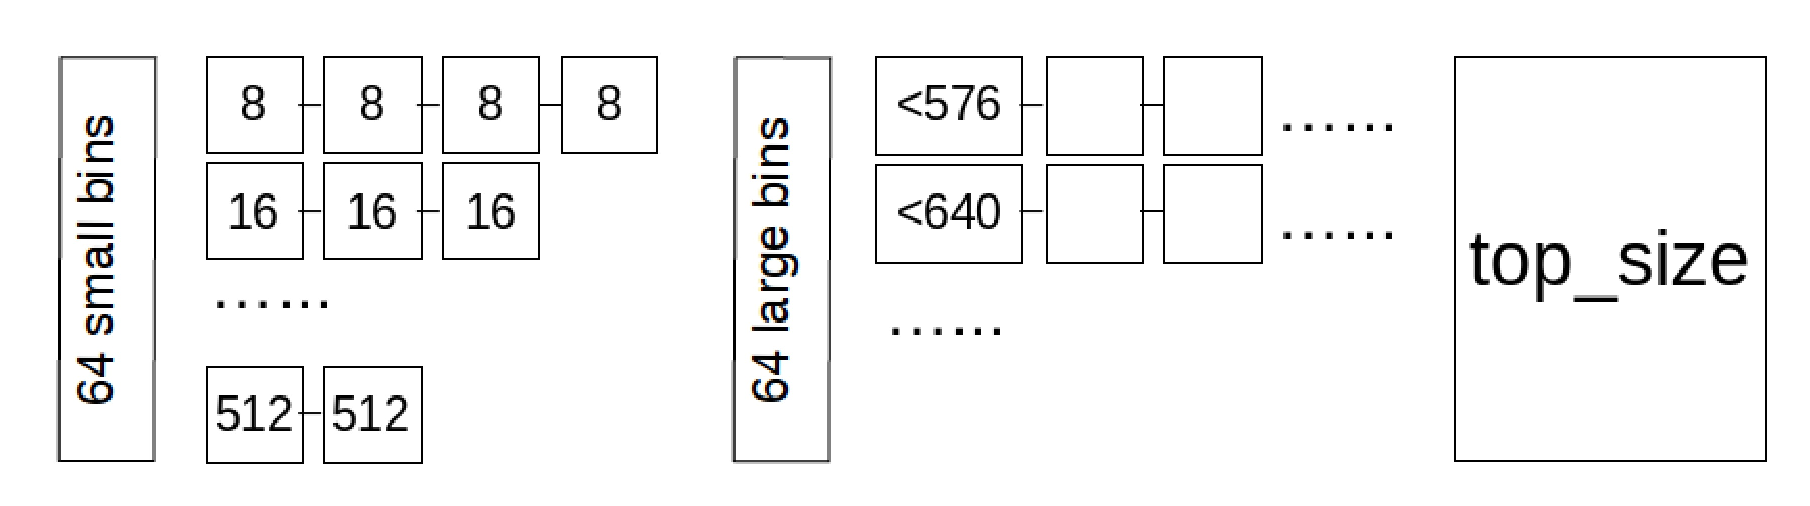
\includegraphics[width=2.4in]{fig7}
\caption{structure of \emph{dlmalloc}}\label{fig_7}
\end{figure}
Each of the segregated lists is called a bin and there are 64 small bins and 64 large bins in \emph{dlmalloc} (Figure \ref{fig_7}). For small bins, each one contains chunks in the exact same size, in which way insertion to or deletion from the list is very quick. For large bins, each bin is associated with a range of sizes and any free chunks within that range are stored in the corresponding bin in the ascending order. So managing large bins is more costly than small bins but fortunately large bins are less frequent than small bins. Apart from these bins, \emph{dlmalloc} also keeps a top chunk, which is always at the end of the heap so that it can be extended or trimmed without affecting other memory chunks. The top chunk is used only when there is no available chunk in any bins that meets the memory request. If the request size is too large to be satisfied from the top chunk and bigger than a pre-defined threshold, \emph{dlmalloc} uses an \emph{mmap}-like system call to allocate this size of memory from the operating system directly. Or it tries to extend the top chunk using \emph{sbrk}-like system call, so that the extended top chunk is big enough to cover the request.
When a chunk is freed by the application, it is put back to one of the bins according to its size, after which \emph{dlmalloc} occasionally coalesces contiguous free chunks to create bigger chunks. If the top chunk is enlarged by combining free chunks next to it, it could be trimmed if it is too large for the need of the application if the freed chunk was mapped directly from the system, it is released to the system immediately. 

% Intruduce the 9 parameters defined in Dlmalloc (1 paragraph)
% draw a table with "para name, type, range, default, comment"
\begin{table*}[htbp]
\centering
\caption{\emph{dlmalloc} parameters}
\label{tab_dlmalloc_parameters}
\resizebox{0.9\textwidth}{!}{
\begin{tabular}{c|c|c|c|c}
\hline
Name & Default & Range & Type & Description\\
\hline
MALLOC\_ALIGNMENT & $2*sizeof(void*)$ & $(1~16)*sizeof(void*)$ & $2^n*sizeof(void*)$ & Alignment unit\\
\hline
FOOTERS & \emph{false} & \emph{true} or \emph{false} & boolean & Additional information of each chunk\\
\hline
INSECURE & \emph{false} & \emph{true} or \emph{false} & boolean & Secure check\\
\hline
NO\_SEGMENT\_TRAVERSAL & \emph{false} & \emph{true} or \emph{false} & boolean & Traversal of chunks before coalescing\\
\hline
MORECORE\_CONTIGUOUS & \emph{true} & \emph{true} or \emph{false} & boolean & Contiguous heap extension support\\
\hline
DEFAULT\_GRANULARITY & 0 & 4~512KB & $2^n$KB or 0 & Unit of heap extension\\
\hline
DEFAULT\_TRIM\_THRESHOLD & 2048KB & 64KB~16MB & $2^n$KB & Threshold of trimming\\
\hline
DEFAULT\_MMAP\_THRESHOLD & 256KB & 16KB~2MB & integer & Threshold of direct memory mapping\\
\hline
MAX\_RELEASE\_CHECK\_RATE & 4095 & 1000~10000 & integer & Frequency of coalescing\\
\hline
\end{tabular}}
\end{table*}


\subsection{Dlmalloc tunable parameters}
As a general-purpose allocator, \emph{dlmalloc} provides several tunable parameters to programmers to adjust at compilation. More specifically, these parameters are defined as macros in the source code, but can be modified via compilers (we achieve that through \emph{gcc}'s ``-D'' flag). In this article, we choose some of these parameters that are more likely to influence the allocator's behavior in terms of memory/time consumption, as our ``victims''. 

One of the core parapemter macros in \emph{dlmalloc}  is \textbf{MALLOC\_ALIGNMENT}. It represents a a multiple of how many bytes all request sizes should be rounded up to. Many of other macros in \emph{dlmalloc} rely on this alignment to avoid any incompatibility. Its default value is $2*sizeof(void*)$ where $sizeof(void*)$ varies across different systems. Normally smaller MALLOC\_ALIGNMENT tends to save more memory but could also cause incompatibility with some applications. 


%For the sake of brevity, only two of them are detailed as examples. \textbf{MALLOC\_ALIGNMENT} is one of the most basic macros in \emph{dlmalloc}, representing a multiple of how many bytes all request sizes should be rounded up to. Most of other macros in \emph{dlmalloc} rely on this alignment to avoid any incompatibility. Its default value is $2*sizeof(void*)$ where $sizeof(void*)$ varies across different systems. Normally smaller MALLOC\_ALIGNMENT tends to save more memory but could also cause incompatibility with some applications. 

\textbf{DEFAULT\_MMAP\_THRESHOLD} is the size bigger than which a request that can not be served via existing free chunks, is allocated through \emph{mmap}-like system call. These \emph{mmap}ed chunks can not be consolidated or reuse by other request, but unlike regular chunks, they never get trapped by other ocuppied chunks, meaning they can be directly released to the system as soon as the application frees it. Bigger DEFAULT\_MMAP\_THRESHOLD tends to cause more memory consumption but save allocation time. The default, 256KB, is ``an empirically derived value that works well in most systems''. A list of the parameters we target in this article is given in Table \ref{tab_dlmalloc_parameters}. More detailed description of these parameters can be found in the comments of \emph{dlmalloc} source code.


%
%In terms of allocation strategies, many researchers have proposed many different strategies for memory allocation and deallocation, which have been well studied and have their own strength and disadvantages\cite{memoryallocatorreview1995}. The basic data structure that most of the allocation strategies use is a linked list of free chunks of memory, which uses a little overhead to store some basic information such as the size of the chunk and whether it is in use, whilst using the free chunk itself to keep the linking pointers. The linked list is also called free list since it only links the unoccupied chunks. Whenever the application issues a memory request, the allocator searches the free list to find a free chunk that meets the request and removes it from the list. When a chunk is freed by the application, it won't be returned to the operating system immediately but inserted to the free list in case the application may soon request a chunk in the same size. A simple example of a free list is depict in Figure \ref{fig_1}, in which the shaded regions represent occupied memory chunks.
%\begin{figure}[htbp]
%\centering
%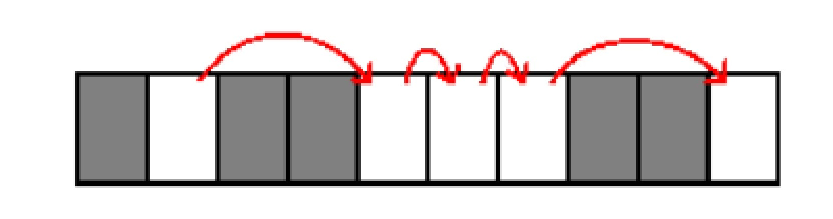
\includegraphics[width=1.5in]{fig1}
%\caption{Basic Linked List}\label{fig_1}
%\end{figure}
%
%\textbf{Sequential fit} is a set of similar allocation strategies including first fit, next fit and best fit. They all use no more than a double linked list to manage the free chunks. When a memory request comes, first fit starts searching the list from the beginning and stops at the first time it meets a free chunk that fulfills the request. It splits the free chunk into two pieces, one of which is in the request size and returned to the application whilst the remainder is inserted back to the list. One big disadvantage of first fit is poor locality, which increases the possibility of cache miss, thus increases the reference time as well as the total running time. Next fit also searches the free list one by one, but starting from where it finds the free chunk for the previous request. The first and next fit both continuously split large free chunks to smaller ones, which cannot be used for later large request, so they both suffer from big fragmentation. The best fit, on the other hand, goes through the whole free list before it makes a decision. So it guarantees to return the smallest free chunk in the list that meets the request, sometimes even the exact fit, hence it performs better in terms of fragmentation than first fit and next fit\cite{Johnstone:1998:MFP:301589.286864}. However, because it goes through the whole list every time there is a request, it costs a lot of time for allocation especially when the free list is very long.
%
%\begin{figure}[htbp]
%\centering
%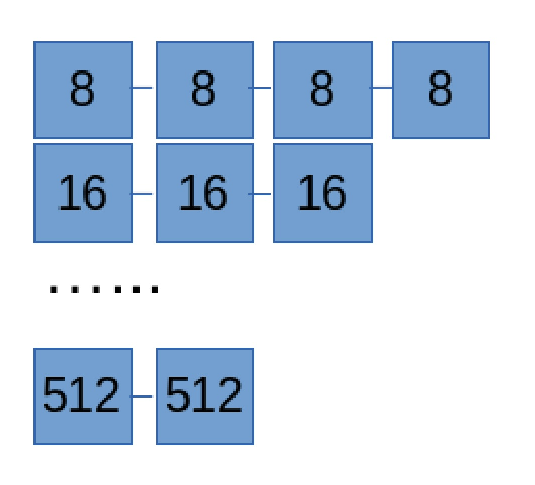
\includegraphics[width=1in]{fig2}
%\caption{Segregated free lists}\label{fig_2}
%\end{figure}
%\textbf{Segregated fit} keeps multiple free lists at the same time (Figure \ref{fig_2}) instead of managing one free list like what sequential fit does. Each of the free lists kept by segregated fit policy contains free chunks in the exact same size which is always a multiple of 8 bytes or a size in power of 2. This has also been known to increase the internal fragmentation (see section \ref{sec_fragmentation}). Each time there is a request of size \emph{n}, it only needs to fetch a free chunk from one of the free lists that corresponds to size \emph{n}. So it saves the allocation time by diminishing the searching time for a best fit whilst keeping a low fragmentation. But it harms a little of the deallocation time since it has to find the exact free list in the deallocated size before the freed chunk can be inserted to that list. What's more, it is possible that there is no available free chunk in the free list that corresponds to the request size, in which case the allocator will get a larger chunk from the next non-empty free list and split the chunk to meet the request. A variant of segregated fit differs only on returning a free chunk without aplitting it even if the chunk is much bigger than the request size. In this allocation strategy, the memory consumption is much higher because each chunk is in a fixed size and may be serving a much smaller request so that the extra size in that chunk can not be reused by other requests. But there is no denying this simplified segregated fit strategy is fast. This also shows there is clearly a trade-off between allocation time and memory consumption.
%
%\textbf{Coalescing} is a strategy which can be combined with or applied to the above allocation strategies, so can the ones introduced later. In order to save memory, most of the policies above choose to split a chunk before returning it to the application. This leads to more and more small chunks that cannot be used for big request. But some of these small chunks could be contiguous in the address space so that they can be concatenated to serve large request, in order to save memory. Coalescing policies try to concatenate contiguous free chunks into a bigger one, but when to apply coalescing remains adjustable in different allocators. This is because if an application request a chunk with size of \emph{n} right after it frees a chunk in the same size, the allocator may have coalesced the freed chunk but split it out from the concatenated chunk again to serve the same-size-request, which is a waste of computation. So instead of coalescing every time the application frees a chunk, some allocators apply coalescing in a fix frequency or once there is no big enough chunk that meets the request. In summary, whether the coalescing policy improves or diminishes the performance of an allocator really depends on the allocator itself and the allocation pattern of the application.
%
%\textbf{Searching strategy} refers to how an allocator manages and searches the free list(s). Some allocators keep the free list(s) in ascending or descending order in terms of address or size. It is quick for searching but may cause poor locality. Good locality refers to trying to allocate chunks that may be accessed subsequently in the application, on the same physical page, in order to minimize the cache misses in the operating system as a means of saving execution time. Searching strategy is quite influential to locality since it determines where subsequent requests should be located. On the other hand, when a chunk is freed and returned to the allocator, there are several ways to place it back in the free list(s), two of which are first-in-first-out (FIFO) and last-in-first-out (LIFO). FIFO strategy gives the most recently released chunk the least priority and places it at the end of the searching queue, whilst LIFO gives the most recently released chunk the highest priority so that it is more likely to be reused in a short time. There is no telling which one is better since it depends on other allocation strategies and the application itself.
%
%\textbf{Bitmap} is another combinable strategy that uses boolean flags to keep the status of chunks or free lists. When it stores the status of chunks, one bit usually represents whether a chunk is in use, and when it keeps the status of free lists, it usually means whether a free list is empty. The bitmap is designed to help the allocator to find an available chunk easily. It narrows the range down by searching the bitmap before searching a free chunk that meets the request.
%
%\textbf{Buddy system} is a well known algorithm which involves a special splitting mechanism. It always allocates memory in several fixed sizes and whenever it needs to split a chunk into two, it splits it in a fixed ratio repeatedly until it meets the smallest chunk that bigger than the request size. In this special splitting mechanism coalescing is fast because finding the other ``buddy'' generated from the same splitting is no more than a couple of simple mathematical computation. Even though the splitting ratio is adjustable, buddy systems still suffer from huge internal fragmentation.
%
%\subsection{Internal and External Fragmentation}
%\label{sec_fragmentation}
%Most of the memory allocators keep all the chunks in the size of multiple of 8 bytes due to the operating system requirements. In these cases, all the memory requests from applications are rounded up to an alignment of 8 bytes before they are really allocated. So the returned chunk is always equal to or slightly bigger than the request size without the applications being aware of it. Then the little extra padding memory is neglected and cannot be used by the applications. This is always refered to as internal fragmentation. On the other hand, at any point of a running application, the memory allocator always hold some free chunks instead of returning them to the operating system, so that it can quickly respond to some memory request from the application using these free chunks. And some of these free chunks may be too small to serve bigger request and for some reason they cannot be coalesced neither (e.g., not next to any other free chunks). The number of these small chunks may increase when the application proceeds, which causes the application occupying more memory than it really needs. This is also known as external fragmentation. 
%
%Allocators always introduce fragmentation, in different degrees. Despite many attempts to minimize memory fragmentation in an efficient way, there is clearly a trade-off between running time and memory fragmentation. For instance allocators with coalescing policies reuse small free chunks by concatenating them whilst introducing more computation for coalescing. And both segregated fit and buddy systems suffer from high fragmentation but they always contribute to fast allocators. 
%
%\subsection{\emph{Dlmalloc}}
%\label{sec_dlmalloc}
%\emph{Dlmalloc} keeps two set of segregated lists for small and large size requests respectively. 
%\begin{figure}[htbp]
%\centering
%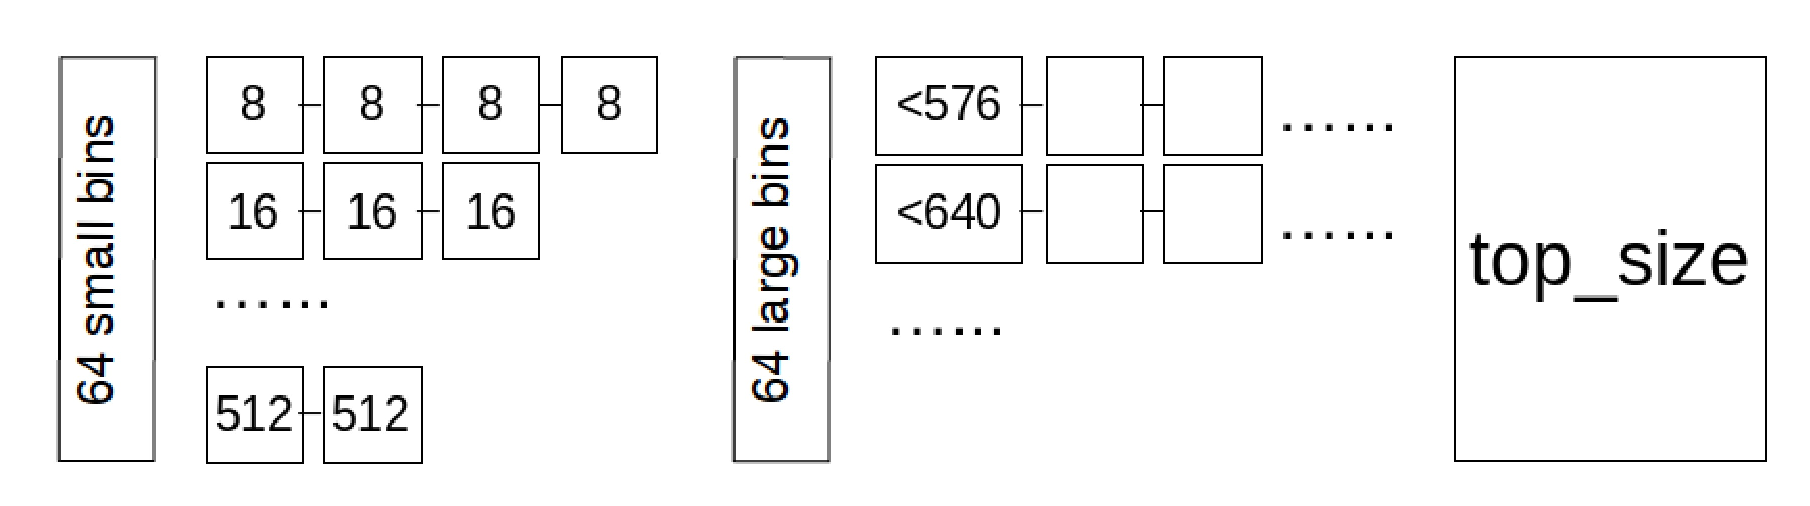
\includegraphics[width=0.4\textwidth]{fig7}
%\caption{structure of \emph{dlmalloc}}\label{fig_7}
%\end{figure}
%Each of the segregated lists is called a bin and there are 64 small bins and 64 large bins in \emph{dlmalloc} (Figure \ref{fig_7}). For small bins, each one contains chunks in the same size aligned to multiple of 8 bytes, which makes the largest chunk in small bins 512 bytes. Since chunks in the same small bin are in the exact same size, there is no need to sort the list, and insertion to or deletion from the list is very quick. For large bins, each bin is associated with a range of size which doesn't overlap with that of other bins. All the chunks larger than 512 bytes are stored in one of the large bins according to its size and kept in ascending order. So finding a chunk with a desired size requires a thorough search of an associated bin in the worst case. Apart from these segregated lists, \emph{dlmalloc} also keeps a top chunk, which is always at the end of the heap so that it can be extended or shrinked without affecting the data structure of other bins. The top chunk is used only when there is no available chunk in any bins that meets the memory request.
%
%\begin{figure}[htbp]
%\centering
%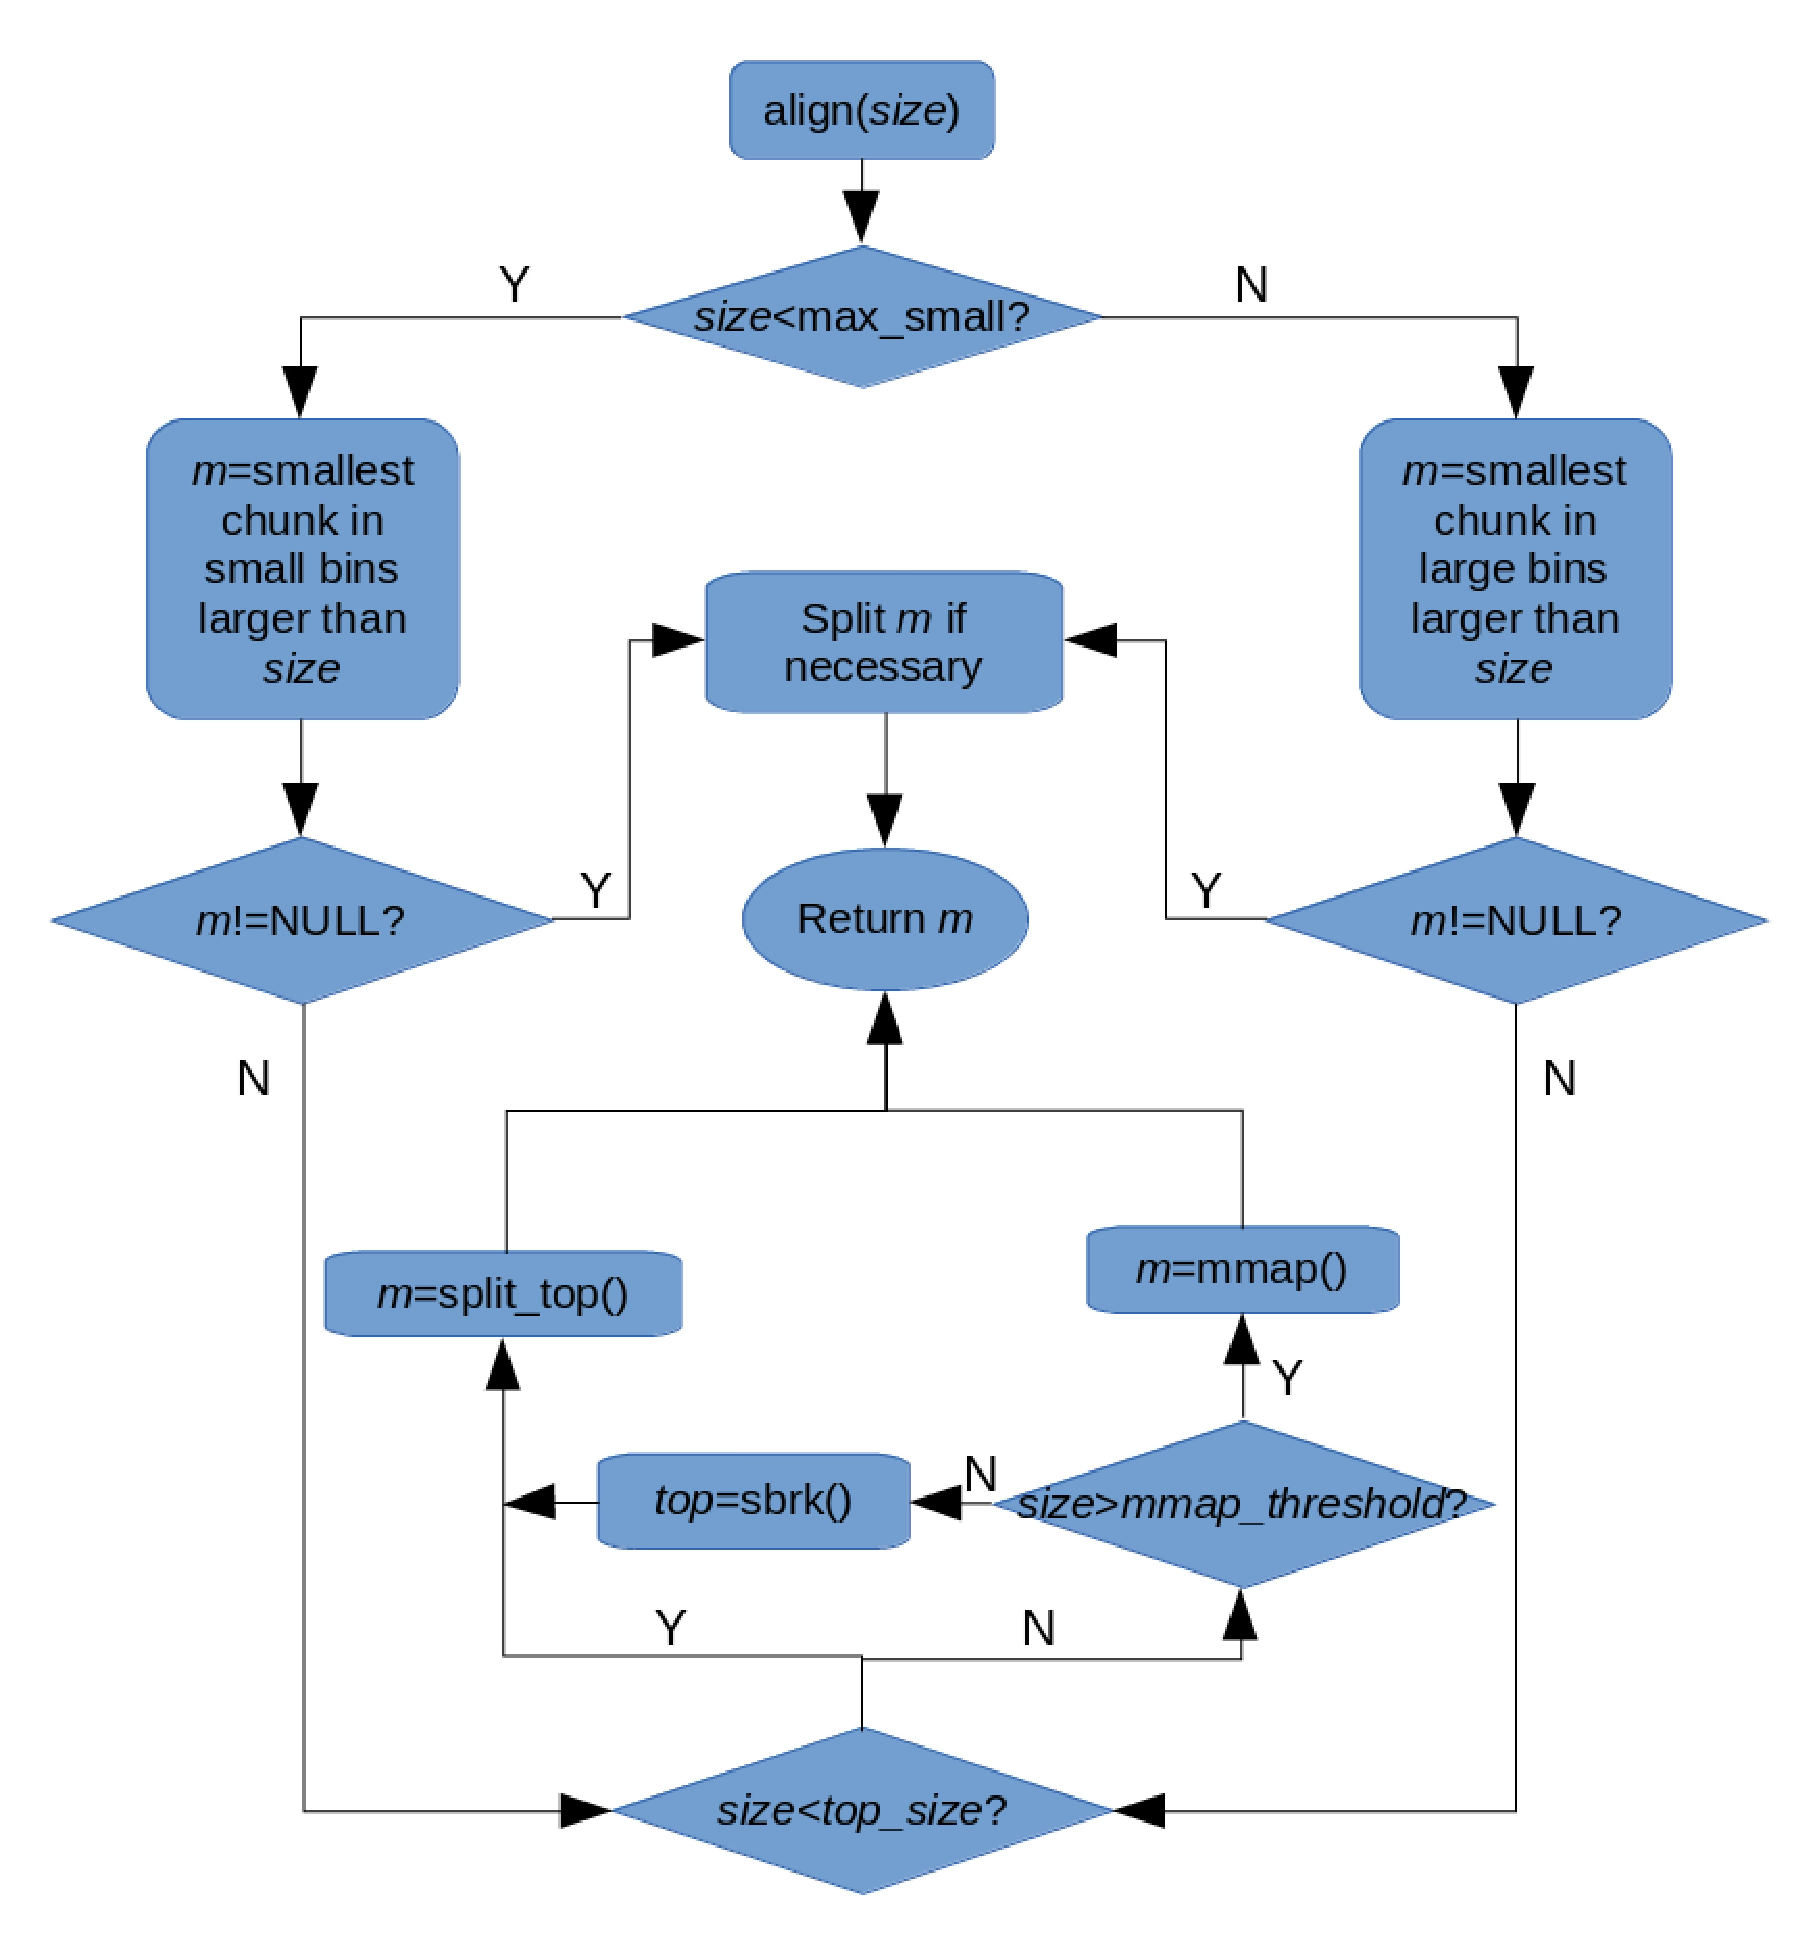
\includegraphics[width=0.4\textwidth]{fig8}
%\caption{allocation process of \emph{dlmalloc}}\label{fig_8}
%\end{figure}
%When a memory request from the application comes, \emph{dlmalloc} first rounds it up to a multiple of 8 bytes, then determine whether it belongs to small or large bins(Figure \ref{fig_8}). Either way, it searches the corresponding bin(s) based on the request size. If an available chunk that meets the requirement is found, it is returned to the application before which split may be applied if necessary. Otherwise, \emph{dlmalloc} tries to use the top chunk to serve the request by splitting the top chunk if the request size is smaller than the size of the top chunk, in which case the remainder is preserved as the new top chunk. If the request size is too large to be gotten from the top chunk, \emph{dlmalloc} uses an \emph{mmap}-like system call to allocate this size of memory from the operating system directly only when the request size is bigger than a pre-defined threshold. Otherwise it tries to extend the top chunk using \emph{sbrk}-like system call, so that the extended top chunk is big enough to cover the request.
%When a chunk is freed by the application, it is put back to one of the bins according to its size, after which \emph{dlmalloc} occasionally coalesces contiguous free chunks to create bigger chunks. If the top chunk is enlarged by combining free chunks next to it, it is also checked whether it is too large for the need of the application, in which case the top chunk may be shrinked. If the freed chunk was mapped directly from the system, it is released to system immediately. 
%There are several other details and techniques in \emph{dlmalloc} that are less relevant to our work, so we don't list them in this article. But they can be easily found in \emph{dlmalloc}'s source code.

%\section{Searching for better DLMalloc parameters}
\section{Deep Parameter Optimisation}

Our approach takes three steps. Firstly we apply Mutation Operators to generate variants of the original \emph{dlmalloc} in order to understand which pieces of the source code could be more influential to the performance. Secondly we analyze the sensitivity of each mutated piece by evaluating the variants on a given set of applications and testsuites. After locating the most interesting and influential part of the code, we expose them to users so that they could be modified from the outside as needed. Thirdly, we apply SBSE approach to find the optimal values for both the existing and exposed parameters for each of the given applications.

This section first discusses how we find and expose interesting parameters.
%** maybe need add some think to justiy the choice of self-implementation. 

\begin{figure}[htbp]
\centering
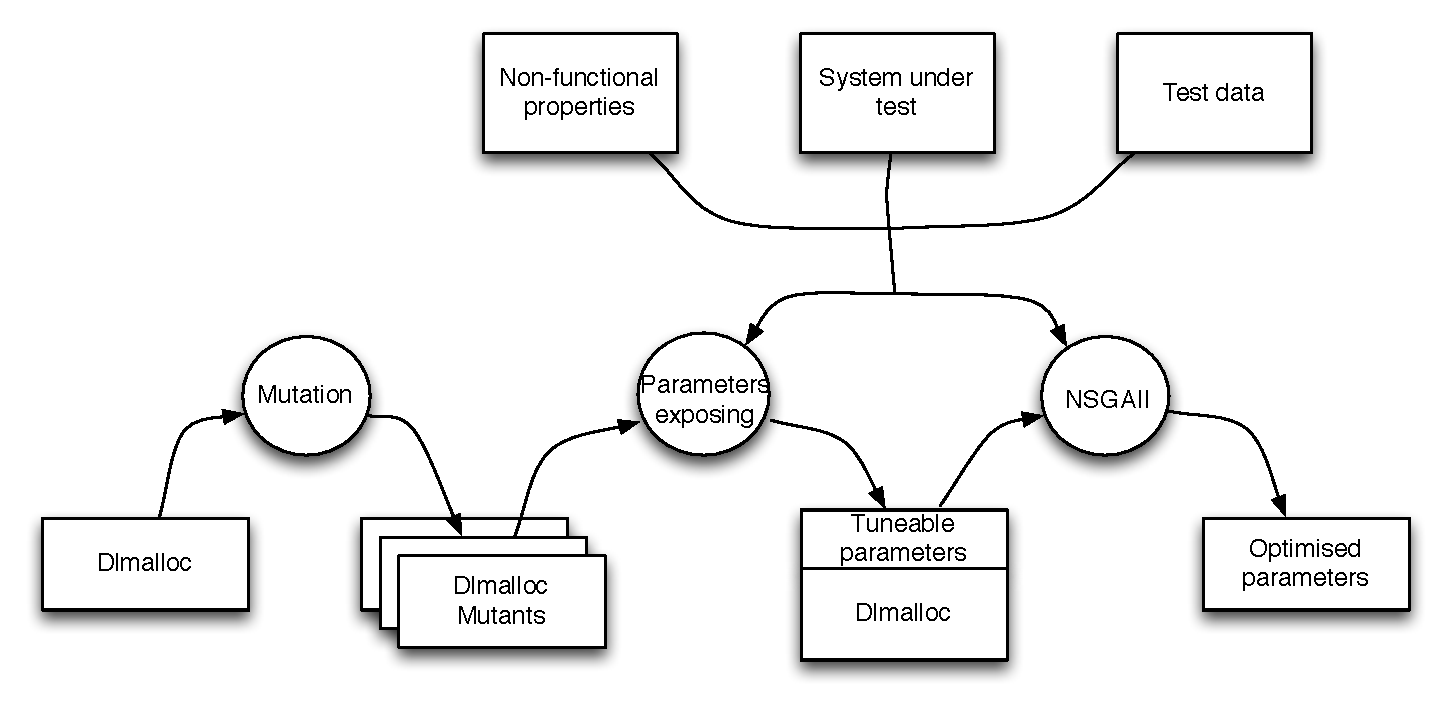
\includegraphics[width=3.2in]{pics/system}
\caption{Deep parameter optimisation workflow}\label{system}
\end{figure}


\subsection{Exposing Implicit Parameters}
Other than the existing parameters introduced above, there might be some other valuable variables which could influence the performance of the allocator but burried and neglected in the massive source code. It could be a constant, an expression or even a predicate. In this paper we try to expose these valuable parts of \emph{dlmalloc} to users so that they can also adjust these parts to fit their needs. Other than blindly exposing random parameters, we need to know how much each piece of code could influence the behavior of \emph{dlmalloc} before we expose it. In another word, we need sensitivity analysis.

% Introduce two types of mutations and why
In order to obtain the sensitivity information, one simple way is to delete each statement at a time to see how important this statement is to the performance of \emph{dlmalloc}. However, when the statement deleted is consist of a very complicated expression, which variable or operator is more important than others remains unknown. A more advanced way to obtain the sensitivity information is via Mutation Operators. Mutation Operators are used in Mutation Testing, which automatically inserts some faults to a target program via Mutation Operators to generate mutants of this program and try to detect those faults using a test suite to see whether the test suite is good enough to reveal program faults. In this work, we just use these Mutation Operators to slightly alter \emph{dlmalloc}, in order to understand which piece of source code influences the memory consumption most. We apply both the statement deletion way and Mutation Operator way in the sensitivity analysis and compare their effectiveness, which is reported later. In either way, there are many variants of original \emph{dlmalloc} generated, all of them only differ from the original in at most one statement. We then evaluate and record the performance of these variants on the subject applications and corresponding test suites. This helps us understand the most influential pieces of code in the original \emph{dlmalloc}.

According to the sensitivity information abtained above, we pick the most influential statements and expose part of them as configurable parameters that can be modified at compilation, just like the other existing parameters introduced in section \ref{sec_dlmalloc_tunable_parameters}. These exposed parameters include constants, expressions and predicates. For constants, exposure is no more than replacing it with a variable that can be defined externally. For expressions and predicates things get a little more compilcated. We obtained different version of an expression or a predicate from the sensitivity information and create a selection statement to include all different versions. In this way, which version of expression or predicate is used can be controled by modifying an external numerical value that controls the selection statement.
% maybe rank


\subsection{MultiObjective Paramter optimisation}
In this work, we apply NSGA II\cite{996017}, a multi-objective Genetic Algorithm, on the searching of the optimal values for those \emph{dlmalloc} parameters list above.
% data representation
Since these parameters can be easily interpreted as integers, we use linear representation to store each candidate, in which each gene is an integer number representing one of the parameters. For mutation, we use different operators according to each gene's legitimate range, while two-point crossover is applied.
% fittness evaluation
Since we need to re-compile \emph{dlmalloc} every time we change the parameters, in order to minimize compilation cost, we only compile \emph{dlmalloc} to a shared object and each application is compiled and linked to that shared object at the beginning of each experiment. In each generation, after new candidates are generated through mutation and crossover operators, each candidate is re-compiled and run with a given subject application. When the performance of the application with each candidate version of \emph{dlmalloc} is collected, an NSGA II style selection is applied to obtain the next generation.
% how to measure time
% how to measure memory
Currently we focus on two non-functional properties: time and memory consumption. \emph{Glibc}'s \emph{wait4} function is used to calculate the cpu time consumed by the application (sum of user time and system time), while we compute the high-water mark of the memory consumption by instrumentation of \emph{dlmalloc}. In this way the memory measured is virtual memory, because the physical pages allocated to an application is not always deterministic but depends on the work load and the system so that measuring the physical memory usage could be hard and misleading.


\section{Experiments}

In order to assess the improvement of our Deep Parameter Tuning approach, we compared our approach with the shallow parameter tuning approach and posed the following research questions: 
 

\begin{description}
 \item[RQ1] {\bf How much improvement can be obtained using the Shallow Parameter Turning approach? }
\end{description}

We asked RQ1 to provide us a baseline results against which to compare the results from our approach. To mimic a traditional Shallow Parameter Turning approach, we used the same NSGAII algorithm introduced in Section \ref{alg} to search for the default explicit parameters for Dlmalloc. To answer this question, we compared the performance of the optimised configuration found by the Shallow Parameter Turning approach with the default Dlmalloc configuration and a set of random generated configurations.  %The default Dlmalloc configuration is chosen by the developer of Dlmalloc and is believed can achieve a good performance on a wide range of programs. We 

\begin{description}
\item[RQ2] {\bf How much more improvement can be obtained using the Deep Parameter Turning approach? }
\end{description}

We ask the RQ2 to see how useful our approach is at find optimised configurations for the given non-functional properties. Our Deep Parameter Turning approach apply NSGAII to optimise both explicit and implicit parameters for Dlmalloc. Of course, should it turn out that the Shallow Parameter Turning approach can find better configuration than our approach, then our approach would not be needed. 

\begin{description}
\item[RQ3] {\bf Do we see evidence that our Deep Parameter Tuning approach can expose implicit parameters which are meaningful to human developer? }
\end{description} 

Should it turn out that the Deep Parameter Tuning approach performs well, achieving much improvement than the Shallow Parameter Tuning approach, then we have evidence to suggest that the mutation based sensitivity analyse used in our approach is able to locate the inner expressions or variables which are sensitive to the given non-functional properties. However, do these inner expressions or variables also make sense to software developer? To answer this research question, we manually investigate the exposed variable and try learn why tuning these parameter can make Dlmalloc more efficient.  

\subsection{Experiment Setup}


\begin{table}[htbp]
\centering
\caption{subject applications}
\label{tab_sub_app}
\resizebox{0.5\textwidth}{!}{
\begin{tabular}{|c|c|c|l|}
\hline
Name & Loc & No. of tests & Type \\
\hline
espresso & 13256 & 19 & Digital electronic gate circuits simplification\\
\hline
cfrac & 6040 & 2 & Big integer factorization\\
\hline
space & 5846 & 3 & Astronautics interpretation\\
\hline
gawk & 45241 & 20 & String processing\\
\hline
\end{tabular}}
\end{table}

For our evaluation, we selected four real world applications: \emph{espresso}, \emph{space}, \emph{cfrac} and \emph{gawk}. \emph{Espresso} is a fast application for simplying complex digital electronic gate circuits and \emph{cfrac} is a factorization application for big integers. We obtain these two applications from the benchmarks of the \emph{DieHard} project\cite{}. \emph{Space} is a well known real world application in astronautics. We obtain this program from the SIR repository \cite{}. \emph{Gawk} is the GNU \emph{awk} implementation for strings processing. We collect this application from the GNU archives \cite{}

Although turning parameter of malloc is less likely to change the behaviour of our subjects under optimise directly, some combination of unusual parameters' values could also crush a subject system. To make sure the configuration generated by our approach always prodcue the same results as the default configuration, we use the number of passed tests as an addtional hard constraints. We used the tests from the \emph{DieHard} project for \emph{Espresso} and \emph{cfrac} and the tests from SIR for \emph{Space}. These tests are designed by programmer and achieve high branche coverage. We mannully generated tests for \emph{awk}, which achieves ** branch coverage. 

All experiments were carried out on a desktop computer with a quad core 3.4GHz CPU and 7.7 GB memory runing 64-bit Ubuntu 13.10. We used \emph{dlmalloc} version 2.8.6 as our base allocator. It was compiled with gcc 4.8.1 with -O3 option. In order to capture the execution time and memory consuming precisly, we adapt developed our own performance tool to measure the CPU time and maxium vitural memory consumption (see Section \label{}) The tool is publicly available at www.fan.put.a.link.later.



\section{Results}
\label{sec_results}

% FIXME: If you can, put a paragraph summarizing this section here so that
% the section heading is not immediately followed by the subsection heading.
% Fan wrote the following.

We formalise the metrics we use to compare multi-objective optimisation approaches in this section.
The results are presented in Section~\ref{sec_answers}, and are used to answer the \textbf{RQ}s.

\subsection{Metrics}
\label{sec_matrics}

To investigate RQ1 and RQ2, we collect the non-dominated set of solutions from each algorithm for 20 runs, and report it in an attainment surface as introduced by Fonseca~\cite{attainment_surface:1996}. To quantitatively compare the quality of each algorithm, we calculate Hypervolume and Contribution indicators to assess the multi-objective Pareto Front.

\textbf{Hypervolume}: The Hypervolume indicator~\cite{797969} measures the space dominated by the solutions. It is defined as the hypervolume of the union of hypercubes dominated by each solution on the Front. The bigger the Hypervolume is, the larger the area dominated by the Pareto Front in the objective space is, and thus the better the performance is.

\textbf{Contribution}: Since there is no way to know the true Pareto Front, we use the non-dominated set of joint solutions from all experiments to approximate the true Pareto Front, forming a `reference' front. The Contribution indicator represents the ratio of solutions on the reference front that are found by a given algorithm. A higher ratio indicates a more successful search. 

To allow comparison across subject programs, objectives are normalised to the original performance of each subject.


\subsection{Answers to RQs}
\label{sec_answers}

\newcommand{\shallow}{Sha}
\newcommand{\all}{All}
\newcommand{\randomsearch}{Rand}
\newcommand{\nsgaii}{NSGA}
\newcommand{\sr}{\emph{\shallow\randomsearch}}
\newcommand{\sn}{\emph{\shallow\nsgaii}}
\newcommand{\dr}{\emph{\all\randomsearch}}
\newcommand{\dn}{\emph{\all\nsgaii}}

For brevity we use \emph{\shallow} to refer to shallow parameters and \emph{\all} to refer to all parameters including shallow and deep parameters, followed by \emph{\randomsearch} or \emph{\nsgaii} to indicate the search method used (random search or NSGA-II). For example, \sn{} refers to using NSGA-II to search for better values for shallow parameters.
%In subsequent graphs, the performance of the original program always locates at (1, 1) since all the performance is normalised to it.

\begin{figure*}[htb]
	\centering
	\subfigure[espresso]{
		\label{fig_attainment_espresso}
		\scalebox{1}{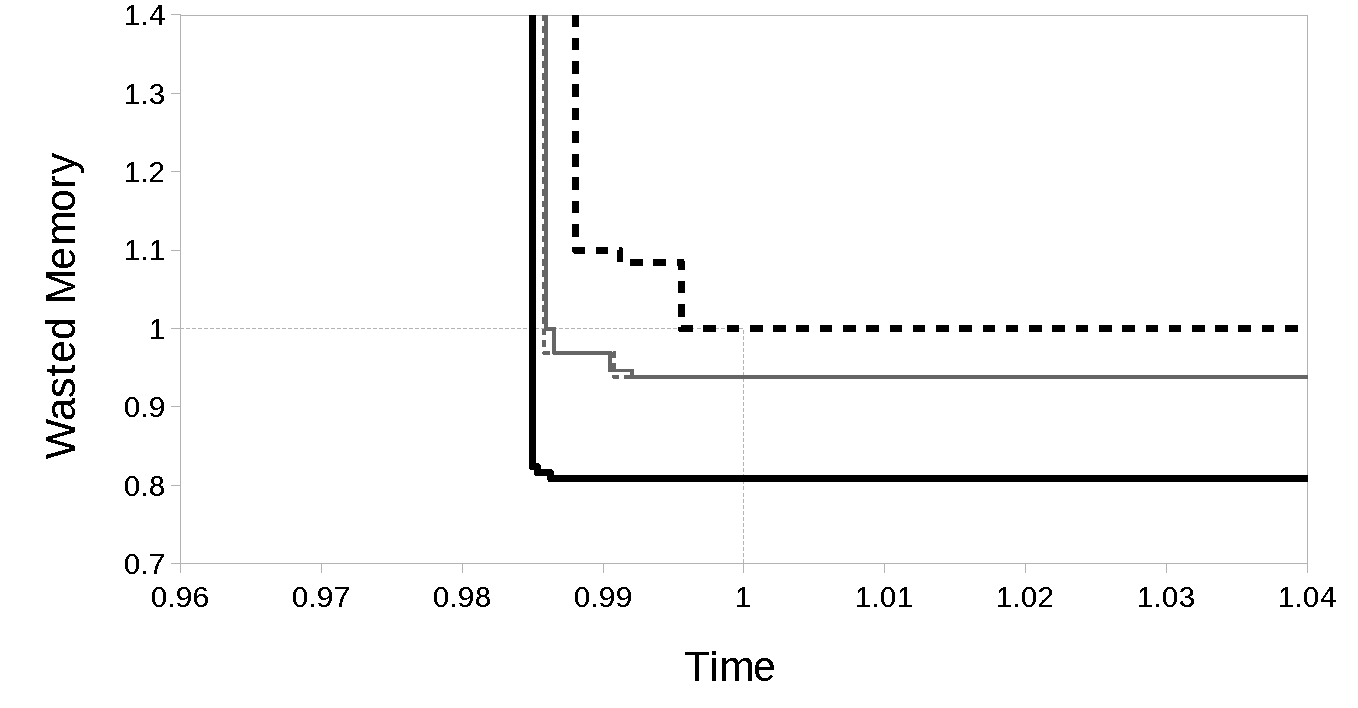
\includegraphics[width=0.47\textwidth]{espresso_attainment_pdf}}
	}
	\subfigure[gawk]{
		\label{fig_attainment_gawk}
		\scalebox{1}{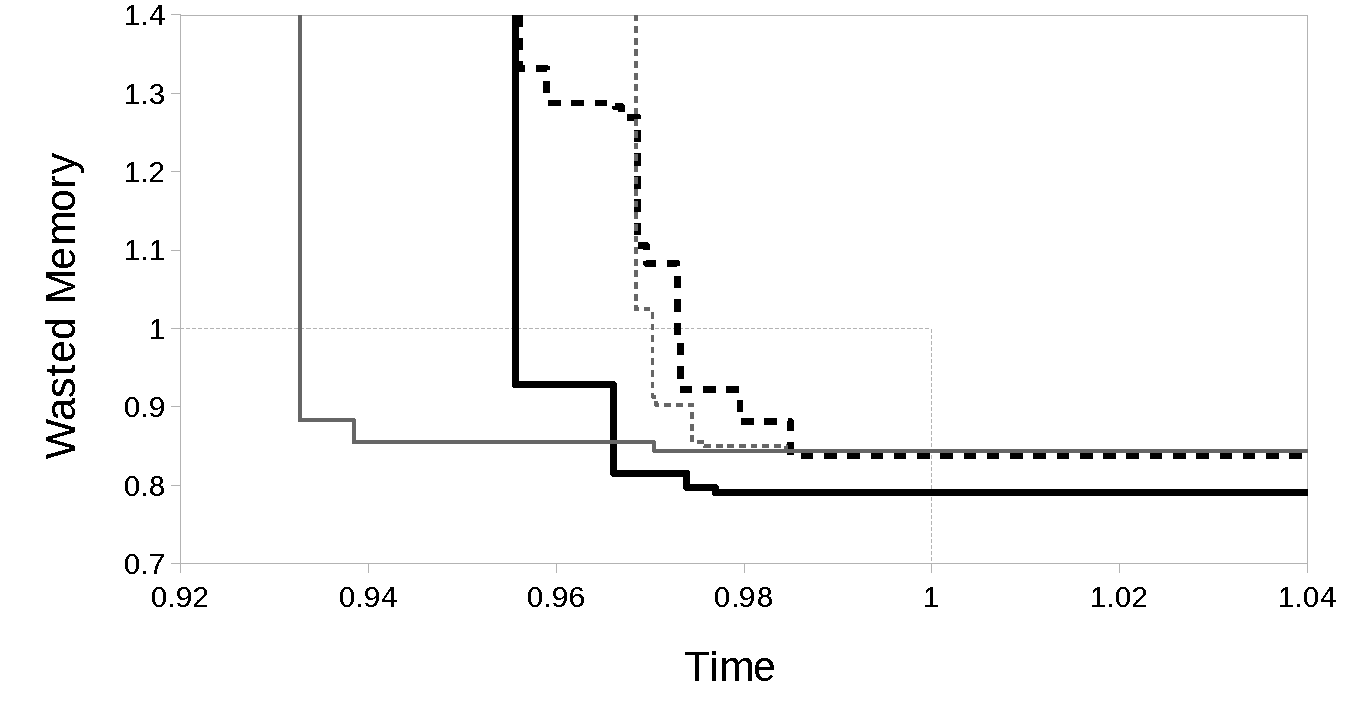
\includegraphics[width=0.47\textwidth]{gawk_attainment_pdf}}
	}
	\subfigure[flex]{
		\label{fig_attainment_flex}
		\scalebox{1}{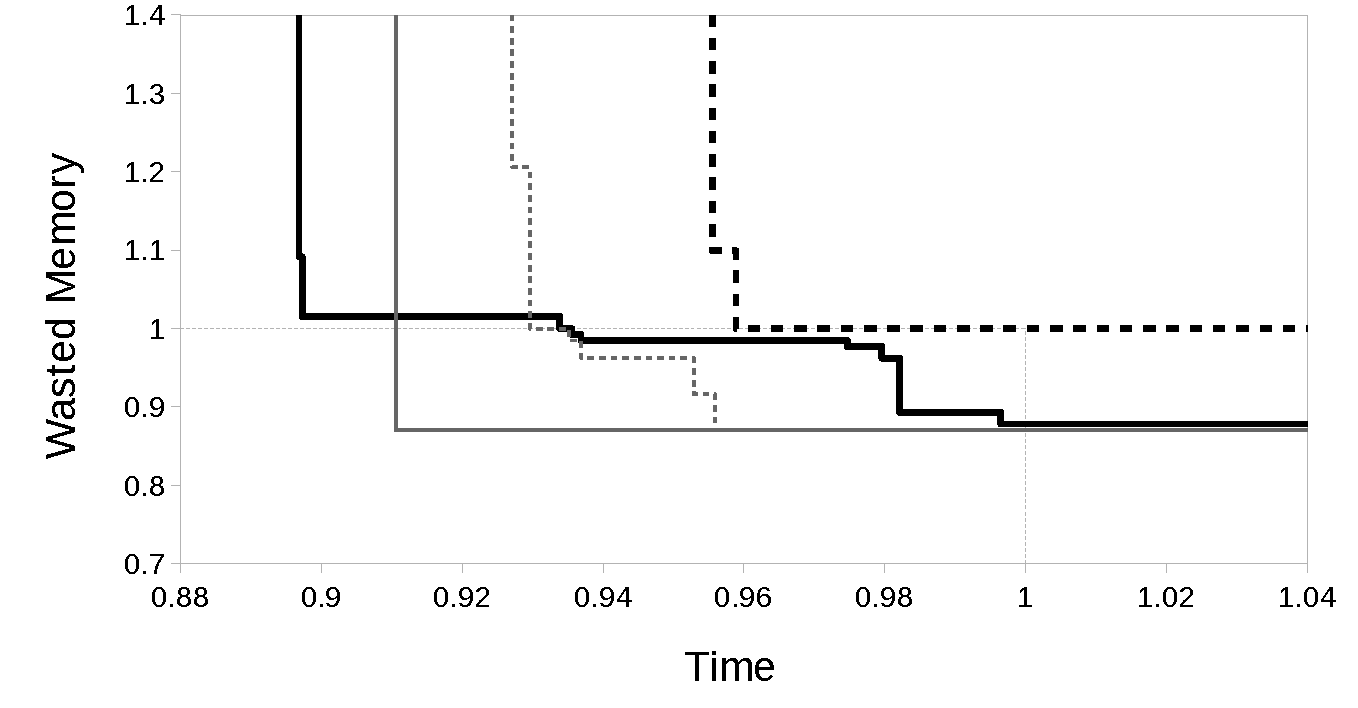
\includegraphics[width=0.47\textwidth]{flex_attainment_pdf}}
	}
	\subfigure[sed]{
		\label{fig_attainment_sed}
		\scalebox{1}{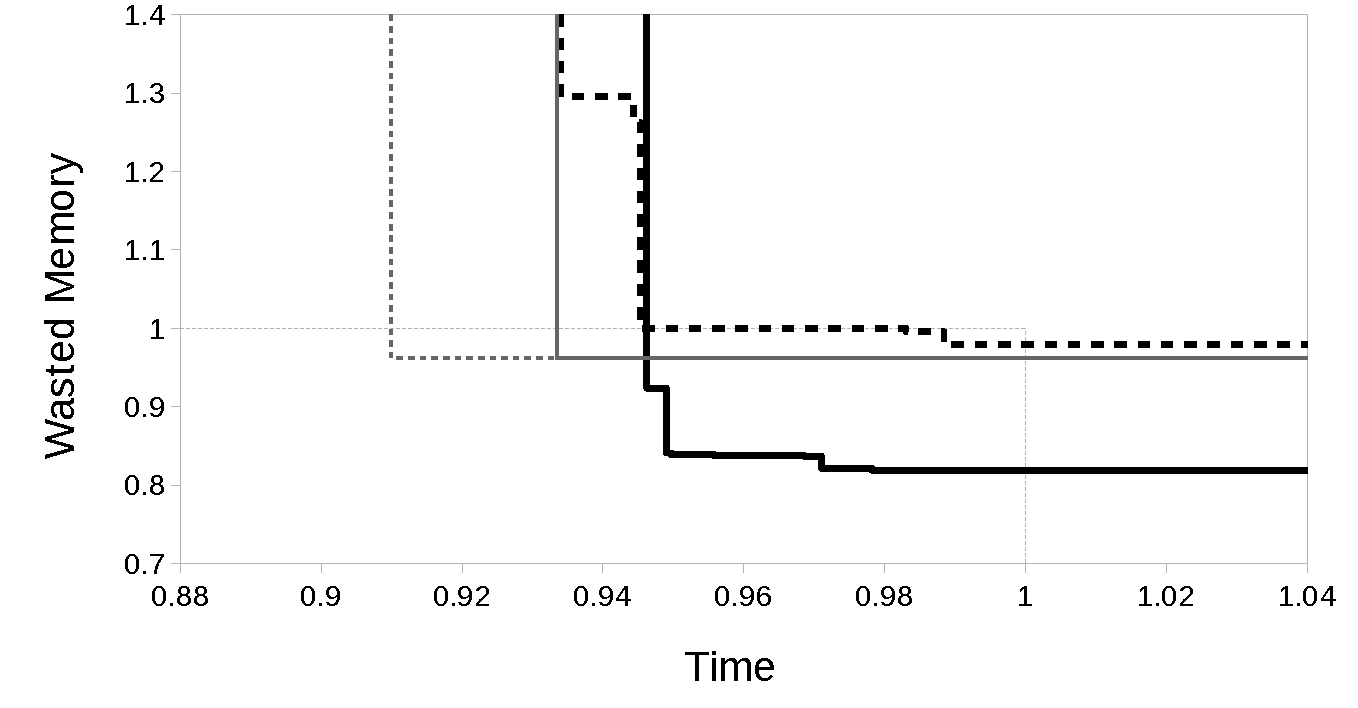
\includegraphics[width=0.47\textwidth]{sed_attainment_pdf}}
	}
	\subfigure{
		\label{fig_attainment_legend}
		
\includegraphics[width=0.45\textwidth]{attainment_legend_pdf}
	}
	\vspace{-1.5em}
	\caption{Combined best solutions from the results of \sr{}, \sn{}, \dr{}, \dn{} over 20 runs for each application. Lower and lefthand solutions dominate high and righthand solutions. `Wasted' memory is memory that is used but not needed.}\label{fig_attainment}

\end{figure*}

To answer RQ1 and RQ2, we first report the 0\%-attainment surfaces (the `reference front' that combines best solutions over all runs) of the results of \sr{}, \sn{}, \dr{} and \dn{} on all subjects in Figure~\ref{fig_attainment}. The solutions are plotted according to their execution time and memory usage (at the `high-water-mark') compared to the original performance. Specially, the original always lies at (1, 1) and is pinpointed by light grey dashed lines. The high-water-mark is our primary target since the remaining non-wasted memory is needed and thus cannot be reduced. 
The figure shows that all algorithms can reduce time or memory consumption without reducing the other objective, implying that the default configuration of \emph{dlmalloc} is not optimal for any application considered. This finding motivates the use of SBSE for tuning memory allocators. In three subjects (\emph{espresso}, \emph{gawk} and \emph{sed}), \dn{} outperforms the other three on memory objective. In terms of time, no algorithm is strictly better and each has its own strengths on different subjects. 
%In Figure~\ref{fig_shallow_random}, we can see that Shallow algorithm is better than Random on subject \emph{sed}, while they are incomparable on the other three subjects. In Figure~\ref{fig_deep_shallow}, Deep algorithm is better than Shallow on three out of four subjects: \emph{espresso}, \emph{gawk}, \emph{sed}, while incomparable on subject \emph{flex}. Notice that unlike other three subjects, Deep can not find solutions have better performance on memory consumption on subject \emph{flex}, and both Shallow and Deep algorithm perform as good as Random, it implies that the optimal solution is very easy to find in the search space. So any search algorithm would fail to ourperform Random search on this special case.

We calculated the Hypervolume and Contribution indicator of each algorithm on every subject, and report them in Figure~\ref{fig_hypervolume} and~\ref{fig_contribution} respectively for all 20 runs. 
In Figure~\ref{fig_hypervolume}, all the values are normalised to the hypervolume of the 0\% attainment reference front, and the closer the value to $1$ is, the better the result is. It is clear that \dn{} outperforms the others on subject \emph{espresso} and \emph{sed} while it performs poorly on subject \emph{flex}, and on subject \emph{gawk} the best value reached by \dn{} is better than that of the others.
%In terms of Hypervolume indicator, Deep algorithm performs the best in general, with an exception on subject \emph{flex}. Shallow algorithm is statistically better than Random on subject \emph{sed}, but there is no significant difference between them on the other three subjects. 
In terms of Contribution, the performance of all algorithms is similar to that of Hypervolume. In general \dn{} is no worse than other algorithms on all subjects but \emph{flex}, where \sn{} has the highest Contribution value.
 
\begin{figure}[htbp]
	\centering
	\subfigure[espresso]{
		\label{fig_hypervolume_espresso}
		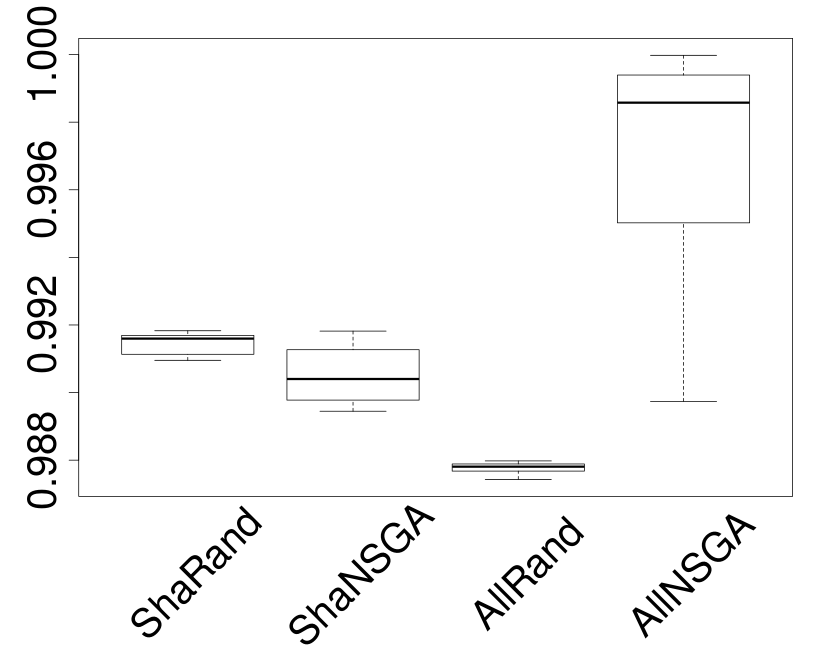
\includegraphics[width=0.22\textwidth]{espresso_hypervolume}
	}
	\subfigure[gawk]{
		\label{fig_hypervolume_gawk}
		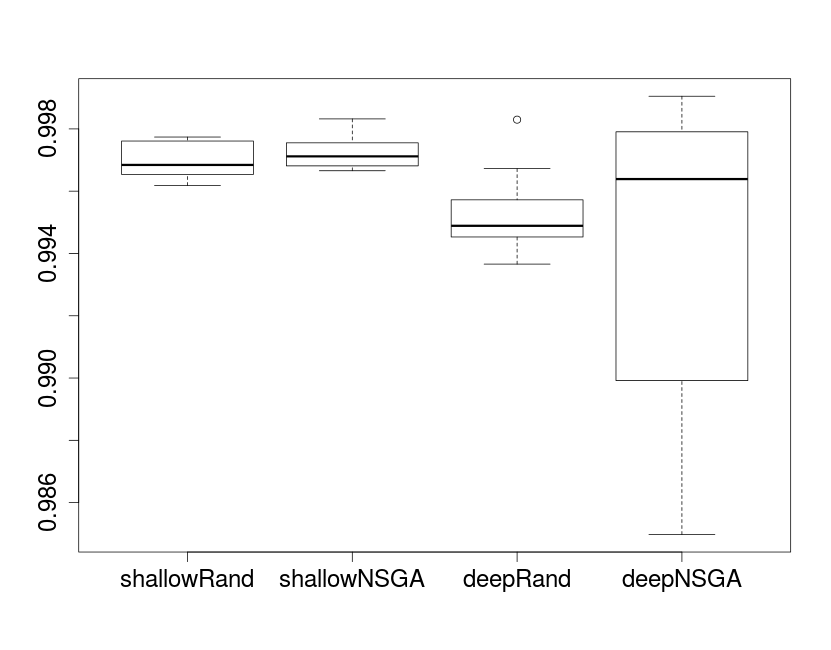
\includegraphics[width=0.22\textwidth]{gawk_hypervolume}
	}
	\subfigure[flex]{
		\label{fig_hypervolume_flex}
		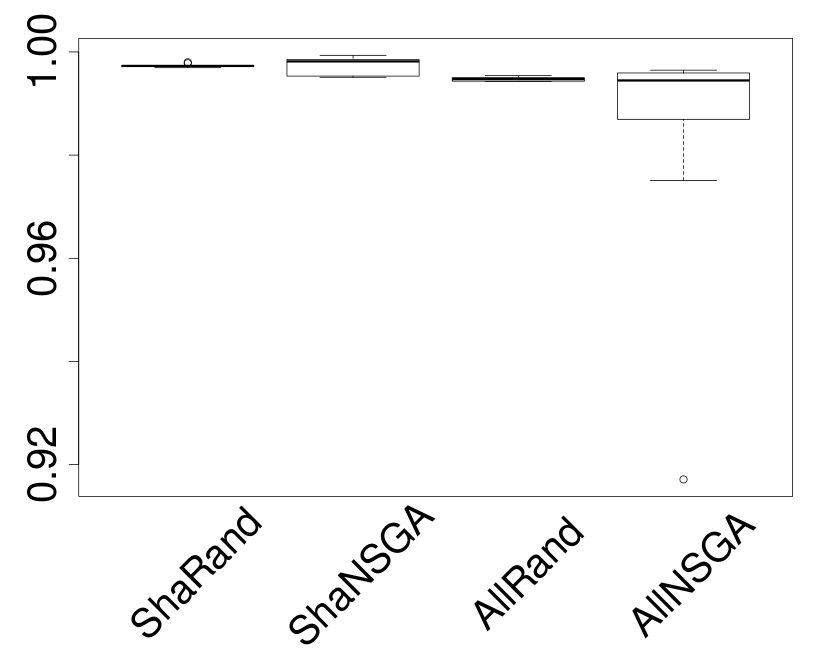
\includegraphics[width=0.22\textwidth]{flex_hypervolume}
	}
	\subfigure[sed]{
		\label{fig_hypervolume_sed}
		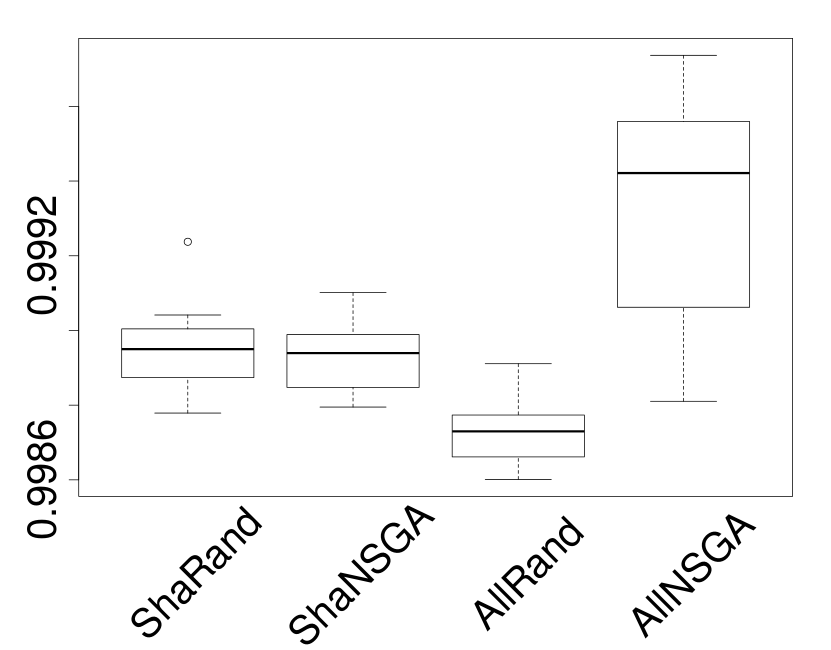
\includegraphics[width=0.22\textwidth]{sed_hypervolume}
	}
	\vspace{-1.2em}
	\caption{Hypervolume indicator of \sr{}, \sn{}, \dr{}, \dn{} on all subjects. Larger values are better.}\label{fig_hypervolume}
	\vspace{-1em}
\end{figure}

\begin{figure}[htbp]
	\centering
	\subfigure[espresso]{
		\label{fig_contribution_espresso}
		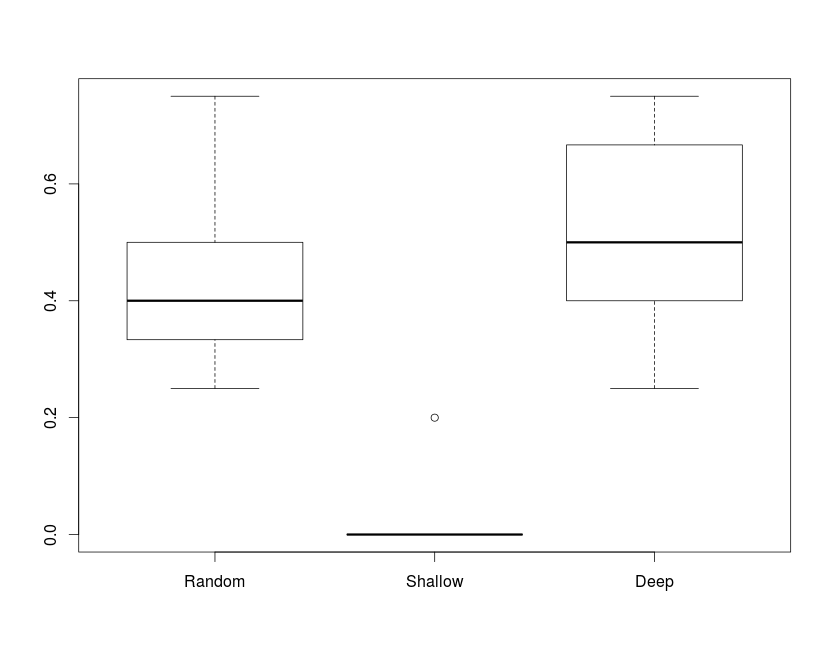
\includegraphics[width=0.22\textwidth]{espresso_contribution}
	}
	\subfigure[gawk]{
		\label{fig_contribution_gawk}
		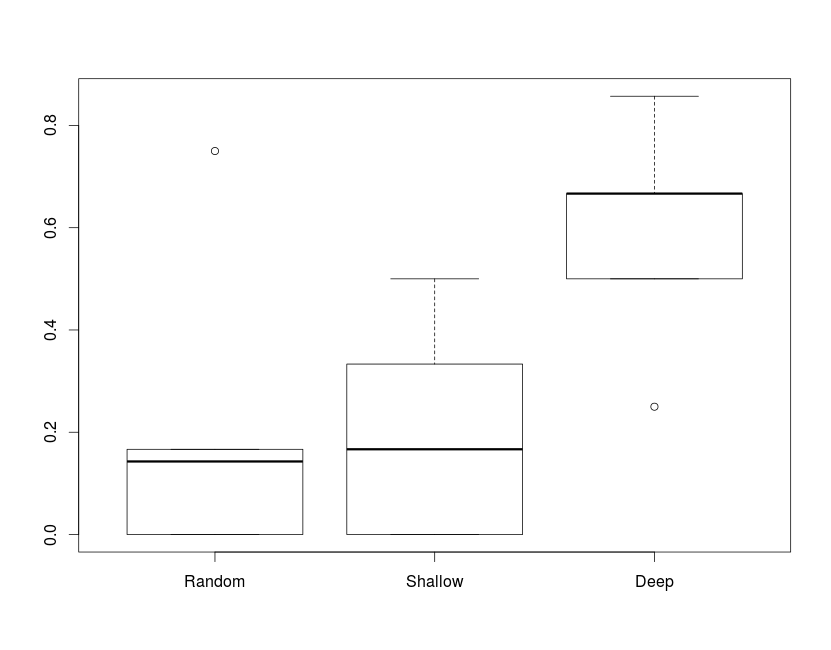
\includegraphics[width=0.22\textwidth]{gawk_contribution}
	}
	\subfigure[flex]{
		\label{fig_contribution_flex}
		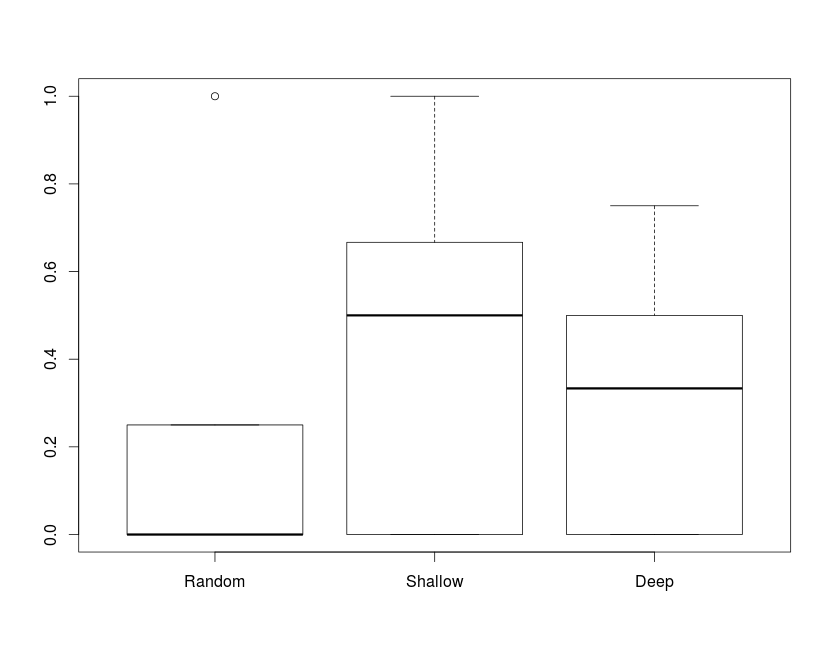
\includegraphics[width=0.22\textwidth]{flex_contribution}
	}
	\subfigure[sed]{
		\label{fig_contribution_sed}
		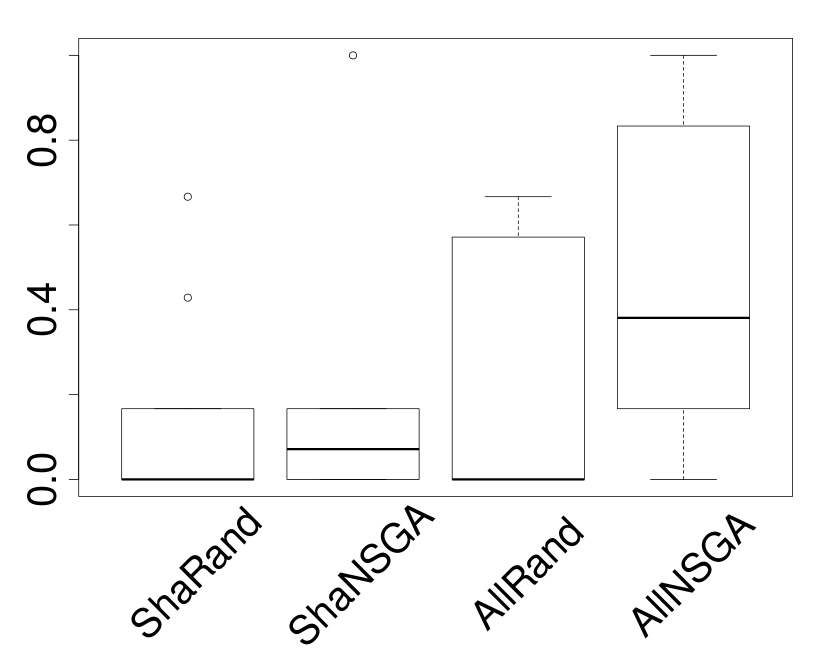
\includegraphics[width=0.22\textwidth]{sed_contribution}
	}
	\vspace{-1.2em}
	\caption{Contribution indicator of \sr{}, \sn{}, \dr{}, \dn{} on all subjects. Larger values are better.}\label{fig_contribution}
	\vspace{-1em}
\end{figure}

\begin{figure}[htb]
	\centering
	\subfigure[espresso]{
		\label{fig_best_time_espresso}
		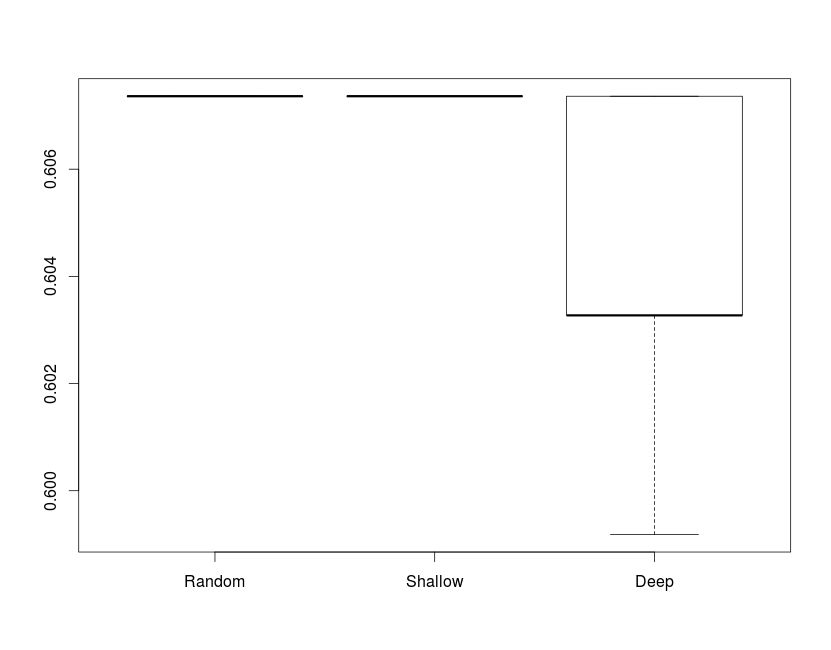
\includegraphics[width=0.22\textwidth]{espresso_best_memory}
	}
	\subfigure[gawk]{
		\label{fig_best_time_gawk}
		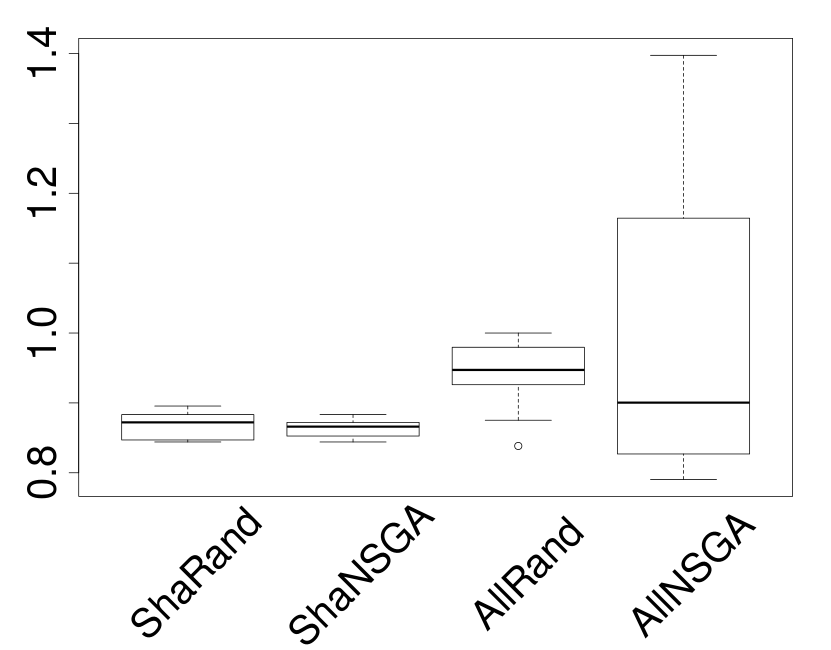
\includegraphics[width=0.22\textwidth]{gawk_best_memory}
	}
	\subfigure[flex]{
		\label{fig_best_time_flex}
		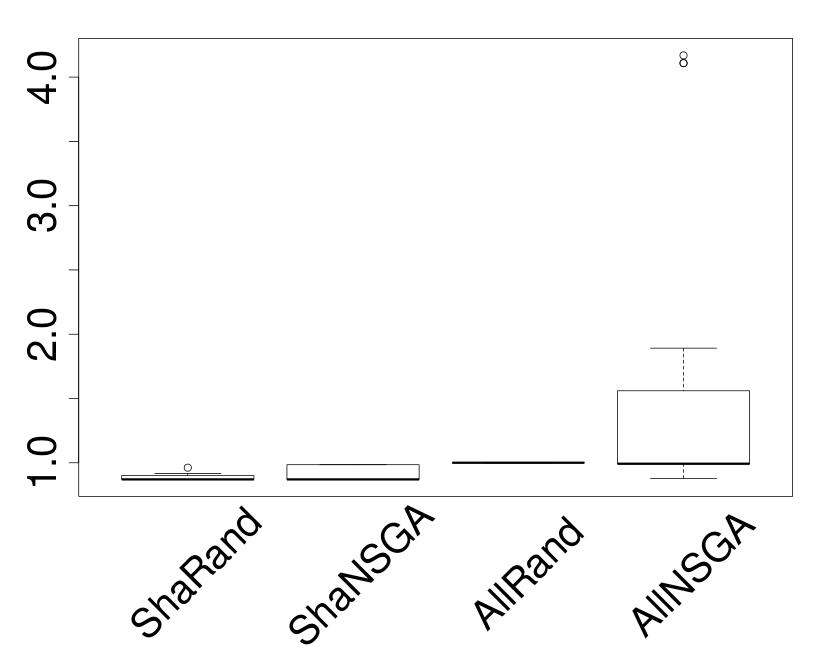
\includegraphics[width=0.22\textwidth]{flex_best_memory}
	}
	\subfigure[sed]{
		\label{fig_best_time_sed}
		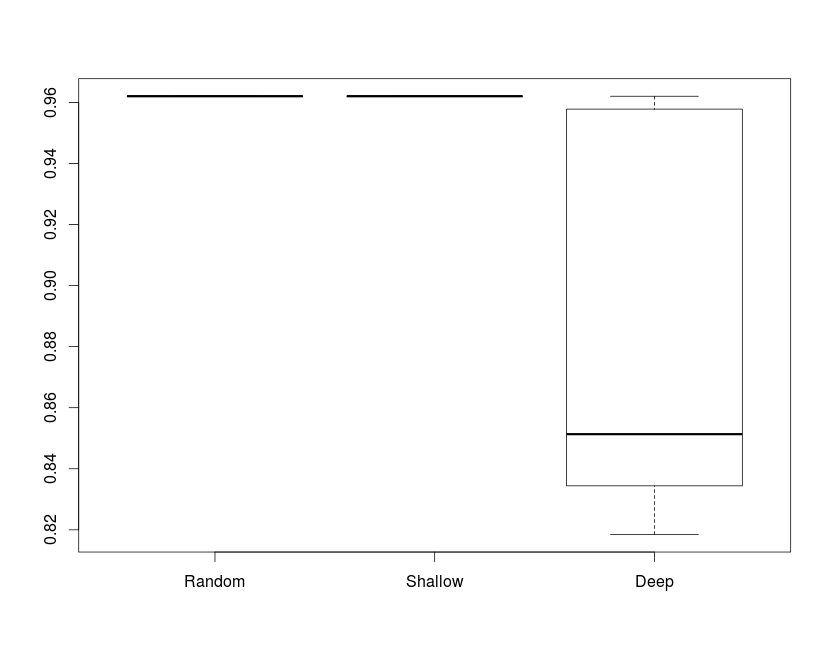
\includegraphics[width=0.22\textwidth]{sed_best_memory}
	}
	\vspace{-1.2em}
	\caption{The least memory consumption found by each algorithm. Smaller numbers are better.}\label{fig_best_memory}
	\vspace{-1em}
\end{figure}

Since \dn{} is good at finding better performance on memory consumption, we report the most memory-saving performance found by each algorithm of each of 20 runs in Figure~\ref{fig_best_memory}. On subject \emph{espresso} and \emph{sed}, \dn{} finds more memory reduction than the other approaches. On \emph{gawk}, it does not perform as consistently, but can also find more memory reduction than other approaches in the best case. 
% FIXME: What does ``potential to do so'' mean here? Please clarify this
% analysis.
% Fan was trying to say, for gawk, though on average AllNSGA doesn't perform as good and stable as other approaches,
% but can occationally outperform other approaches.

%Statistics tests are applied to Hypervolume, Contribution and Best-Memory-Reduction over all subjects.
%We choose Wilcoxon \emph{U}-test because we don't make any assumption on the distributions and the experiments are not paired.
%Considering four approaches on four subjects, we apply Bonferroni Correction (16 tests) to draw conservative conclusions.
%For those \emph{p}-values less than $5\%/16=0.3125\%$, we apply
%Vargha-Delaney effect size measure ($\hat{A}_{12}$) and report the effect sizes in Table~\ref{table_p_value}.
%The effect sizes are all large (effect size larger than $0.79$ or less than $0.21$).

Inferential statistical tests were applied to the Hypervolume, Contribution and Best-Memory-Reduction results over all subjects.
We used the Mann-Whitney-Wilcoxon \emph{U}-test since we make no assumptions about results distributions and apply a Bonferroni Correction (catering for 16 total statistical tests) to draw conservative conclusions with no risk of Type 1 error.
For those \emph{p}-values less than $0.05/16=0.003125$, we apply the
Vargha-Delaney ($\hat{A}_{12}$) effect size measure (see Table~\ref{table_p_value}).
The effect sizes are all large (either above $0.79$ or below $0.21$).

In all experiments involving \emph{\all{}*} we generated and evaluated invalid
configurations (i.e., those that that cause the program to crash). However,
this issue is not specific to our deep-parameter approach: 
surprisingly, even by just tuning the programmer-specified shallow parameters 
(\sr{} and \sn{} optimisations) we {\em also} encounter (and discard) some
configurations that crash the program.
%Unlike shallow parameters, deep parameters are exposed from internal
%sub-expressions that were not monitored or protected by the programmers,
%hence they are expected to cause crashes more often. As a result, the valid
%configurations are sparser in the search space. 
This suggests that SBSE memory allocator tuning can be used as a search based testing technique \cite{mh:icst14-keynote}.
Without any guidance, \dr{}
finds valid configurations less often than \sr{}, and thus requires more
optimisation time than \sr{}. Holding the searches to the same budget means
that \dn{}, which must explore a higher search space, will exhibit a higher
variance. 
% This is also the reason why the performance of \dn{} is not alway
% stable on all subjects. 
Despite this more challenging search space, exposing and optimising deep
parameters still allows \dn{} to find better configurations
than \sn{}.

\begin{table*}[htb]
\centering
\caption{Vargha-Delaney effect sizes of Hypervolume, Contribution and Best Memory Reduction for any two of the approaches on all subjects. Only the effect sizes of tests with \emph{p}-value less than $5\%/16=0.3125\%$ are reported.}
\label{table_p_value}
\resizebox{0.85\textwidth}{!}{
\begin{tabular}{|l|l|r|r|r|r|r|r|r|r|r|r|r|r|}
\hline
\multicolumn{2}{|l|}{\multirow{2}{*}{Comparing Approachs}} & \multicolumn{4}{c|}{Hypervolume}                                                                             & \multicolumn{4}{c|}{Contribution}                                                                            & \multicolumn{4}{c|}{Best Memory Reduction}                                                                   \\ \cline{3-14} 
\multicolumn{2}{|l|}{}                           & \multicolumn{1}{c|}{\emph{espresso}} & \multicolumn{1}{c|}{\emph{gawk}} & \multicolumn{1}{c|}{\emph{flex}} & \multicolumn{1}{c|}{\emph{sed}} & \multicolumn{1}{c|}{\emph{espresso}} & \multicolumn{1}{c|}{\emph{gawk}} & \multicolumn{1}{c|}{\emph{flex}} & \multicolumn{1}{c|}{\emph{sed}} & \multicolumn{1}{c|}{\emph{espresso}} & \multicolumn{1}{c|}{\emph{gawk}} & \multicolumn{1}{c|}{\emph{flex}} & \multicolumn{1}{c|}{\emph{sed}} \\ \hline
\multirow{3}{*}{\dn{}}              & \dr{}        & 1.000                     & --                        & --                        & 0.975                    & 0.859                     & --                        & --                        & 0.835                    & 0.000                     & --                        & --                        & 0.000                    \\
                                   & \sn{}        & 0.935                     & --                        & 0.105                     & 0.808                    & 0.868                     & --                        & 0.191                     & 0.868                    & 0.063                     & --                        & 0.950                     & 0.050                    \\
                                   & \sr{}        & 0.900                     & --                        & 0.035                     & 0.785                    & 0.814                     & --                        & --                        & 0.875                    & 0.100                     & --                        & 0.979                     & 0.050                    \\ \hline
\multirow{2}{*}{\dr{}}              & \sn{}        & 0.000                     & 0.053                     & 0.038                     & 0.045                    & --                        & --                        & 0.144                     & --                       & 1.000                     & 0.940                     & 1.000                     & 1.000                    \\
                                   & \sr{}        & 0.000                     & 0.070                     & 0.000                     & 0.040                    & --                        & --                        & --                        & --                       & 1.000                     & 0.928                     & 1.000                     & 1.000                    \\ \hline
\multicolumn{1}{|c|}{\sn{}}         & \sr{}        & 0.198                     & --                        & --                        & --                       & --                        & --                        & --                        & --                       & 0.800                     & --                        & --                        & --                       \\ \hline
\end{tabular}
}
\vspace{-1.5em}
\end{table*}

To enable a more quantitative look at maximal time and memory savings, we
examine the extreme performance observed in our experiments. We report
those that have the best performance on
one objective, even at the cost of reducing performance on the other
objective, found by each
algorithm on each subject and summarise them in Table~\ref{table_best_time_memory}.
Some of these results are significant
departures from the original and are thus not plotted in Figure~\ref{fig_attainment}. 

\begin{table*}[htb]
\centering
\caption{Best reduction of time or memory (separately) found by each algorithm}
\label{table_best_time_memory}
\resizebox{\textwidth}{!}{
\begin{tabular}{|c|r|r|r|r|r|r|r|r|r|r|}
\hline
\multirow{2}{*}{Subject} & \multicolumn{1}{c|}{\multirow{2}{*}{\begin{tabular}[c]{@{}c@{}}Time\\ Original (s)\end{tabular}}} & \multicolumn{4}{c|}{Time Reduction (\%)} & \multicolumn{1}{c|}{\multirow{2}{*}{\begin{tabular}[c]{@{}c@{}}Memory Original\\ (Peak/Wasted KB)\end{tabular}}} & \multicolumn{4}{c|}{Wasted Memory Reduction (\%)} \\ \cline{3-6} \cline{8-11} 
                         & \multicolumn{1}{c|}{}                                                                               & \sr{}  & \sn{}  & \dr{}  & \dn{} & \multicolumn{1}{c|}{}                                                                                            & \sr{}    & \sn{}    & \dr{}    & \dn{}    \\ \hline
\emph{espresso}                 & 7.24                                                                                                & 1.4      & 1.4      & 1.5     & 1.5     & 3500/521                                                                                                         & 6.1        & 6.1        & 0          & 19.2       \\ %\hline
\emph{gawk}                     & 3.43                                                                                                & 3.2      & 6.7      & 4.4      & 4.4     & 29680/3552                                                                                                       & 15.6       & 15.6       & 16.2       & 20.9       \\ %\hline
\emph{flex}                     & 0.13                                                                                                & 7.9      & 10.0      & 6.2      & 11.6    & 10816/525                                                                                                        & 13.0       & 13.0       & 0          & 12.2        \\ %\hline
\emph{sed}                      & 0.25                                                                                                & 9.4      & 7.0      & 7.0      & 5.4     & 7048/948                                                                                                         & 3.8        & 3.8        & 2.1          & 17.9       \\ \hline
\end{tabular}
}
\vspace{-3mm}
\end{table*}

To answer RQ3, we provide the average optimisation computation time for each of the apporaches in Table~\ref{table_computation_time}. Recall that \dr{} generates and evaluates numerous invalid configurations. However, since crashing or incorrect mutants can be discarded immediately, the computation time of \dr{} is the lowest among all approaches (given a fixed budget in terms of mutants considered). Similarly, \dn{} generates invalid configurations more often than \sn{}, so it costs less computation time than \sn{}. Taking the deep parameter discovery time into account, \dn{} requires slightly more time than \sn{} does, and the percentage of the extra computation time is reported in the last column of Table~\ref{table_computation_time}. Ultimately, \dn{} requires at most 18\% more computation time than \sn{} (on \emph{espresso}), but requires only 0.7\% more computation time on \emph{flex}, on which \dn{} does not perform as well as \sn{}. Overall, since this optimisation step is a compile-time rather than run-time cost and can be done before deployment, we view the benefits of deep parameter optimisation as significantly outweighing their slight additional optimisation time cost.

\begin{table}[h]
\centering
\vspace{-1.4em}
\caption{Computation Cost in Time}
\label{table_computation_time}
\resizebox{0.47\textwidth}{!}{
\begin{tabular}{|c|r|r|r|r|r|r|}
\hline
\multirow{2}{*}{Subject} & \multicolumn{4}{c|}{Optimisation Time (h)}                                                                        & \multicolumn{1}{c|}{\multirow{2}{*}{\begin{tabular}[c]{@{}c@{}}Exposing\\ Time (h)\end{tabular}}} & \multicolumn{1}{c|}{\multirow{2}{*}{\begin{tabular}[p{2cm}]{@{}c@{}}Extra Time Needed\\ for \emph{*\nsgaii} (\%)\end{tabular}}} \\ \cline{2-5}
                         & \multicolumn{1}{c|}{\sr{}} & \multicolumn{1}{c|}{\sn{}} & \multicolumn{1}{c|}{\dr{}} & \multicolumn{1}{c|}{\dn{}} & \multicolumn{1}{c|}{}                                                                             & \multicolumn{1}{c|}{}                                                                                                           \\ \hline
\emph{espresso}                 & 39.7      & 46.4     & 9.0      & 39.3     & 12.5                                                                                                    & 18.5                                                                                                                          \\ %\hline
\emph{gawk}                     & 22.7      & 18.4     & 13.9     & 16.4     & 5.4                                                                                                     & 11.7                                                                                                                          \\ %\hline
\emph{flex}                     & 7.7       & 6.3      & 5.3      & 5.0      & 1.3                                                                                                     & 0.7                                                                                                                           \\ %\hline
\emph{sed}                      & 9.4       & 7.6      & 5.9      & 6.6      & 1.9                                                                                                     & 12.6                                                                                                                          \\ \hline
\end{tabular}
}
\vspace{-1em}
\end{table}


\subsection{Threat to Vadility}

Currently, the deep parameters are chosen manually according to the sensitivity information. We take the top 10, 100, 300 most influential mutants and investigate which line of code has been mutated most often in these mutants, then expose the mutated part of these lines as deep parameters. It remains a possibility that this way of choosing exposed parts could be sub-optimal. It is also possible that there exists some other parts of code, which could be influential to the memory and/or time consumption, slipped away from our approach. 

Despite less possible, the repeating times of the experiments might be insufficient to statistically support the claims. 

The choose of test suite could in some degree affect the results. Even with a good test suite that achieves a high branch coverage, it could still differ from the distribution of the real world inputs, in which case the optimized configuration over this test suite may not achieve the best performance in the real world. On the other hand, if we could find and optimize a piece of code that will be executed in most of the real inputs, we are likely able to achieve better performance in terms of the real world scenario.

One other concern is whether the result holds on other applications. Despite subject applications from different fields for different uses, potential threat to our conclusion could exist beyond our test. Currently we can only claim that our approach works on the applications under test in this paper, but because of the wide range of where these applications come from, it is highly likely this approach can be easily generalized to other applications and lead to similar result on many of them.

\section{Related Work}

Some embedded systems, especially those executing multimedia applications, suffer from massive memory usage and limited resources. Risco-Martin et al\cite{Risco-Martin:2009:ODM:1569901.1570116}\cite{RiscoMartin2010572} decomposes memory allocators into several components, for each of which there are several optional implementations of different allocation strategies. Combining different implementations to generate the optimal dynamic memory manager (DMM) becomes a searching problem. They use grammatical evolution to solve this optimization problem with two real world applications: Physics3D and VDrift. The results show that, on average their custom DMM reduces memory accesses by 23\%, memory consumption by 38\% and energy usage by 21\%, comparing with the state-of-the-art dynamic memory managers currently used by these applications. Other than \emph{dlmalloc}, they target on the DMM on embedded systems which run memory-intensive application. In their approach, they try to find the best combination of several basic strategies, different from which, we start from the state-of-the-art combination of allocation strategies and adjust its configuration to each application. 

Grunwald and Zorn introduced \emph{CustoMalloc}, a system that customizes and synthesizes a memory allocator for a given application\cite{SPE:SPE4380230804}. The basic idea is, run an application and record all the memory allocation and deallocation during the run so that \emph{CustoMalloc} can find the most frequent sizes. Then the system generates a custom memory allocator using two allocation strategies for different sizes: fast but more overhead way for the most frequent sizes and normal way for other sizes. As the results show, the synthesized allocators are uniformly faster than the Berkeley UNIX allocator whilst being more memory efficient. They also reported that the performance of a synthesized allocator is not sensitive to the input of the application, suggesting that for a given application, the memory allocation and deallocation patterns for different inputs are similar. 

Because general-purpose memory allocators may not meet the programmer's expectation on some specific applications and writting custom memory allocators from scratch is difficult and error-prone, Berger et al\cite{Berger:2001:CHM:381694.378821} introduced an infrastructure for customizing memory allocators using C++ templates and inheritance. In this infrastructure, there are different components that are sufficient to generate a custom memory allocator for programmers to choose, so that generating a new custom memory allocator is simple and easy without any additional programming cost. The results show that the performance of the customized memory allocator is comparable to \emph{dlmalloc}, one of the best uniprocessor allocators. The contribution of this work is simplifying the process of creating a custom memory allocator and minimizing the human effort.

Since improving the locality of a memory allocator can improve the memory reference speed, there are allocators developed to do so. Jula et al\cite{Jula2007} present a container-oriented memory allocator, \emph{Defero}. In \emph{Defero}, the upper level of its allocation strategy is segregated fit. But instead of double linked list, in the lower level it uses trees to store the free chunks using the context of containers as hints. \emph{Defero} always tries to allocate a new object ``close'' to another related object to improve the memory reference locality. In order to use the semantic-rich context of C++ Standard Template Library (STL) containers, only a little modification to STL container is needed. What's more, it also provides some tunable parameters for users to customize the allocator. The results show that the applications under test perform better with \emph{Defero} than those using GNU STL allocator. They also report how the tunable parameters influence the performance of \emph{Defero}.

Another locality-improving memory allocator, \emph{Vam}, is introduced by Feng and Berger\cite{Feng:2005:LDM:1111583.1111594}. It also uses segregated fit as its upper level allocation strategy, but saves the overhead in small size chunks by allocating them on the same page. For other sizes of chunks, it applies a little more overhead to preserve their locality information. The results show that \emph{Vam} performs 4\%-8\% better than \emph{dlmalloc} on general applications.

Continuing on locality improving works, Jula et al\cite{Jula:2009:TMA:1542431.1542447} present two memory allocation schemes: \emph{Two Partition} (\emph{TP}) and \emph{Medius}. They both use K-regions method to keep the location information, which is used as a hint in the first attempt of allocation. Then they use the traditional size-based method to allocate the memory if the first attempt fails. The difference between \emph{TP} and \emph{Medius} is that, \emph{Medius} allows the chunks within the same K-region in different sizes whilst \emph{TP} doesn't. Then the authors compare \emph{TP} and \emph{Medius} with some other allocators including \emph{dlmalloc} and \emph{Defero}, then report and analyze the empirical results on 7 applications.

By combining most of the allocation strategies introduced previously, Hasan et al\cite{Hasan20061051} proposed a tunable hybrid memory allocator. Similar to \emph{dlmalloc}, Hasan's memory allocator uses two sets of allocation strategies for different sizes. For large requests, it manages a double linked list on which best fit strategy with deferred coalescing is applied. And for medium and small sizes, it uses segregated lists to manage the free chunks less than 1KB. What's more, it also uses a bitmap to track the emptiness of these segregated lists so that finding a non-empty free list is accelerated. A little different from serving medium requests, Hasan's allocator additionally keeps a quick list for small sizes, to which the freed chunks in small sizes are inserted before being coalesced or put back to segregated lists. The quick list is an unsorted single linked list and all the small chunks in it keep their in-use bit set. The idea is that the most common request sizes are 32 bytes or less\cite{Zorn:1992:EMS:142181.142200} so that keeping them in a quick list saves allocation time. This allocator also applies several different coalescing strategies in different scenarios, the details of which can be found in their paper. According to their results, their memory allocator performs 11-54\% better in terms of running time, compared with \emph{dlmalloc}, whilst maitaining nearly equal memory consumption.

Berger et al\cite{Berger:2002:RCM:583854.582421} generalize a general-purpose region-based allocator called \emph{reaps}, which combines the region semantics into general-purpose allocator. They show that their \emph{reaps} outperforms other allocators including some using region-like semantics. They also replace some custom allocators in their applications with \emph{dlmalloc} and show that most of the custom memory allocators perform no much better than \emph{dlmalloc}, and those who significantly outperform \emph{dlmalloc} are all \emph{reaps}-like allocators. They claim that, ``Our results indicate that programmers needing fast regions should use reaps, and that most programmers considering custom allocators should instead use the Lea allocator''.

Speaking of parameter tuning, there has been many works studying the influence of algorithms' configuration or automatically adjusting it, including \emph{ParamILS}\cite{hutter2009paramils}. \emph{ParamILS} is an automatic framework proposed by Hutter et al, which automatically configures an algorithm's parameters to get the best performance on a given test suite. It uses a local-search-based algorithm to look for the optimum and gets the fitness by running the application with each candidate configuration. Since long running time of an application leads to unbearable evaluation cost, \emph{ParamILS} uses a novel technique which adaptively controls the cut-off running time of each trial, to adjust the evaluation time. Their results show that, they achieved consistent performance improvements using \emph{ParamILS}.

Hoffmann and Sidiroglou et al\cite{Hoffmann:2011:DKR:1961296.1950390} proposed \emph{PowerDial}, a system which dynamically adjusts application's behavior to make it adaptable to fluctuating working load and power. It first transforms some configuration parameters to non-constant variables residing in the application's memory, so the behavior of the application can be altered by controling these variables when the application is running. Then it pre-runs the application with each possible configuration to abtain how these parameters influence the application, memorizes the Pareto-best candidates in terms of application's non-functional properties and the quality of the output. Whenever \emph{PowerDial} detects a resource shortage it sacrifices some of the output quality by changing the values of those variables according to its record, to prevent the application from crashing. After the resource crisis has passed, it automatically recover those values so that the application can go back to its original trace. The experimental resutls show that \emph{PowerDial} can enable four benchmark applications to survive power caps effectively.

\section{Conclusions}
In this paper, we use Shallow Parameter Tuning to adjust a general-purpose memory allocator, \emph{dlmalloc}, to each of the given applications. In this experiment, multi-objective optimization is applied considering applications' time and memory consumption. It turns out that by Shallow Parameter Tuning, the best general-purpose memory allocator can be improved on a specific application. Beyond that, we expose more tunable parameters from the original program according to the sensitivity information derived from evaluating Mutation-Operator-generated variants. By tuning these deep parameters, we are able to find richer solutions on the Pareto front. (**sumarize other results later) By statistically analyzing the results, we believe the Deep Parameter Tuning is an effective and interesting approach that worth further investigation.

%\end{document}  % This is where a 'short' article might terminate

%ACKNOWLEDGMENTS are optional
\section{Acknowledgments}
**Acknowledgement. Grant.

%
% The following two commands are all you need in the
% initial runs of your .tex file to
% produce the bibliography for the citations in your paper.
\bibliographystyle{abbrv}
\bibliography{myReading}  % sigproc.bib is the name of the Bibliography in this case
% You must have a proper ".bib" file
%  and remember to run:
% latex bibtex latex latex
% to resolve all references
%
% ACM needs 'a single self-contained file'!
%
%APPENDICES are optional
%\balancecolumns

\balancecolumns
% That's all folks!
\end{document}
